% !TeX program = xelatex
\documentclass[UTF8,11pt,a4paper]{ctexart}

\usepackage[a4paper,margin=2.35cm]{geometry}
\usepackage{amsmath,amssymb,bm}
\usepackage{booktabs,longtable,array,tabularx}
\usepackage{enumitem}
\usepackage{xcolor}
\usepackage{graphicx}
\usepackage{siunitx}
\usepackage{hyperref}
\usepackage{cleveref}
\usepackage{fancyhdr}
\usepackage[most]{tcolorbox}

\hypersetup{
  colorlinks=true,
  linkcolor=blue!55!black,
  citecolor=green!40!black,
  urlcolor=cyan!45!black,
  pdftitle={从零理解平面双足机器人 FDDP 与 FIR-QP-MPC 项目},
  pdfauthor={MSc Biped FDDP Project}
}
\sisetup{detect-all}
\setlist{nosep,leftmargin=2em}
\setlength{\parindent}{2em}
\setlength{\parskip}{0.35em}
\pagestyle{fancy}
\fancyhf{}
\fancyhead[L]{平面双足机器人项目学习指南}
\fancyhead[R]{FDDP + FIR-QP-MPC}
\fancyfoot[C]{\thepage}

\newcommand{\code}[1]{\texttt{#1}}
\newcommand{\pass}{\textcolor{green!45!black}{\textbf{PASS}}}
\newcommand{\fail}{\textcolor{red!65!black}{\textbf{FAIL}}}
\newcommand{\boundary}{\textcolor{orange!70!black}{\textbf{边界}}}
\newcommand{\partialstatus}{\textcolor{orange!75!black}{\textbf{PARTIAL}}}
\newcommand{\pending}{\textcolor{blue!60!black}{\textbf{PENDING}}}

\newtcolorbox{intuitionbox}{colback=blue!3,colframe=blue!45!black,title=直观理解}
\newtcolorbox{projectbox}{colback=green!3,colframe=green!40!black,title=本项目怎样做}
\newtcolorbox{evidencebox}{colback=orange!4,colframe=orange!65!black,title=证据与结果}
\newtcolorbox{warningbox}{colback=red!3,colframe=red!55!black,title=常见误解与边界}

\title{\textbf{从零理解我的平面双足机器人项目}\\[0.4em]
\large 从建模、FDDP、MuJoCo 到 FIR-QP-MPC、接触同步与鲁棒性验证}
\author{面向零基础读者的项目讲解文档}
\date{2026 年 7 月 19 日}

\begin{document}
\maketitle

\begin{abstract}
本文假设读者此前不了解双足机器人、最优控制或模型预测控制，从“机器人为什么会倒、怎样把走路拆成可以求解的问题”开始，沿着本项目真实开发顺序解释模型、离线 FDDP 名义轨迹、MuJoCo 独立重放、C0/C1/C2 在线控制、故障安全和统计鲁棒性。每个算法先讲直觉，再给最少但必要的公式，随后指出它在本项目中的代码入口、输入输出、实验结果与不能夸大的边界。本文档独立于论文 \code{v4.tex}，既可从头学习，也可用于组会、论文写作和答辩复习。事实以 2026 年 7 月 19 日当前代码和机器可读 YAML/CSV 为准。
\end{abstract}

\begin{center}
\fbox{\parbox{0.92\linewidth}{
\textbf{必须先记住的 claim boundary：}
当前项目已支持 \textbf{accepted 10-step FDDP planning/contact + full MuJoCo replay + integrated C0/C1/phase-only/C2-final ablation}。硬件接口概念是
$\bm q_{\mathrm{cmd}}=\bm q_{\mathrm{ref}}+\Delta\bm q$；
$\bm\tau_{\mathrm{ref}}$ 只用于 FDDP planning/analysis，不是位置舵机 torque command。
当前十步 FDDP trajectory 已通过 planning/contact feasibility gates；完整 \SI{10}{s} MuJoCo replay 的 20/20 个自然接触事件按序匹配；四模式同协议消融、$\pm\SI{4}{N}$ 双方向 30-seed recovery、15 类 fault injection 和 32 场景 $\times$ 30 seeds 的 statistical robustness 均通过，正式矩阵为 960/960。
因此可以声称“当前定义的核心软件与仿真验收链已经完成”。但现有 E6 timing 仍是短样本历史证据，并非 100,000-update hard real-time proof；真实串口通信、舵机标定、支撑保护下的实机站立/行走也尚未完成。任何地方都不得写成“真实硬件已经自主行走”。
}}
\end{center}

\tableofcontents
\clearpage

\section{这份文档怎样读}\label{sec:reading}

\begin{intuitionbox}
第一次读时不要先背 FDDP、FIR 或 QP 的定义。先把项目看成一句话：\textbf{先离线计划一条能走的名义动作，再在执行时用小幅位置修正抵抗俯仰扰动，并按真实触地时刻调整播放进度。}
\end{intuitionbox}

\begin{itemize}
  \item \textbf{零基础路线：}按目录顺序阅读。先理解机器人、坐标、关节和位置舵机，再进入 FDDP、MuJoCo、C0/C1/C2。
  \item \textbf{组会路线：}先读第~\ref{sec:one_sentence}节、第~\ref{sec:pipeline}节、第~\ref{sec:gaps}节和第~\ref{sec:oral}节，再回看需要解释的算法。
  \item \textbf{论文路线：}重点阅读模型、FDDP、十步重放、控制器消融、鲁棒性与参考文献；所有具体数字都回到对应 YAML/CSV。
\end{itemize}

\begin{warningbox}
“仿真通过”不等于“硬件必然成功”。仿真证明的是在当前模型、扰动集合和验收门槛内，软件输出有限、轨迹可重放且统计试验通过；舵机方向、机械间隙、电源、串口延迟、地面摩擦和三维侧向稳定仍需要实机验证。
\end{warningbox}

\section{先用一句话理解整个项目}\label{sec:one_sentence}

这个项目把“走路”拆成两个时间尺度：

\begin{enumerate}
  \item \textbf{Offline FDDP} 使用非线性刚体动力学、接触约束和代价函数，先在计算机里求出一条 nominal trajectory；
  \item \textbf{Online FIR-QP-MPC} 不重新求完整步态，而是根据 MuJoCo 中测得的 torso pitch error 快速计算小的 joint-position correction $\Delta\bm q$；
  \item 最终位置命令是
  \begin{equation}
      \bm q_{\mathrm{cmd}}(k)=\bm q_{\mathrm{ref}}(k)+\Delta\bm q(k).
      \label{eq:qcmd}
  \end{equation}
\end{enumerate}

FDDP 负责“计划应该怎样动”，C0 检查“只回放计划会怎样”，C1 负责“受到 pitch disturbance 后怎样修正”，C2 负责“实际触地时刻与计划时刻不同后怎样重新对齐参考相位”。

\begin{table}[htbp]
\centering
\caption{第一次阅读时应先建立的模块分工}
\begin{tabularx}{\linewidth}{@{}p{2.25cm}X p{3.0cm}@{}}
\toprule
模块 & 在本项目中做什么 & 当前证据层级 \\
\midrule
FDDP & 离线求 nominal state/control trajectory 与固定 contact schedule & 10-step planning/contact gates 通过 \\
MuJoCo & 用 position-actuator proxy 检验 nominal 在另一动力学模型中的可回放性 & 完整 10-step replay 通过，20/20 events matched \\
C0 & 直接回放 $\bm q_{\mathrm{ref}}$，作为无在线修正基线 & 已验证 \\
C1 & FIR prediction + QP 计算 pitch-recovery correction $\Delta\bm q$ & 10-step IAE 相对 C0 改善 10.79\% \\
C2-final & C1 correction + event-type local-leg phase synchronisation & 10-step timing error 相对 C1 改善 38.16\% \\
Robustness & 对扰动、摩擦、坡度、台阶、延迟、增益和噪声做 batch comparison & 32 场景、960/960 trials，正式 gate 通过 \\
Runtime & 加载 nominal/controller artifact 并按周期输出 position command & runtime-loadability；非硬件 walking \\
\bottomrule
\end{tabularx}
\end{table}

\section{先理解为什么这件事难：机器人为什么会倒}\label{sec:why_hard}

\begin{intuitionbox}
人走路时会提前抬脚、把身体重心送向支撑脚，并在脚落地早了或晚了时立刻调整。双足机器人没有这种天然反射：它必须从模型、传感器和控制程序中得到相同的信息。只要重心、触地时刻或关节动作略有偏差，误差就会在下一步继续积累。
\end{intuitionbox}

本项目主要处理三类困难：

\begin{enumerate}
  \item \textbf{非线性动力学：}关节角度、速度和力矩之间不是简单比例关系；一条腿摆动也会带动躯干。
  \item \textbf{接触切换：}双脚着地、单脚支撑、另一脚落地是不同的动力学模式；触地会产生瞬时冲击。
  \item \textbf{模型与执行差异：}规划器中的理想机器人与 MuJoCo、位置舵机以及未来真实硬件不可能完全一样。
\end{enumerate}

所以项目不是“写一个 FDDP 程序就结束”，而是建立一条证据链：先证明 nominal 在规划模型里可行，再证明它能在独立仿真器中通过位置命令重放，最后证明在线修正、触地同步、安全状态和批量扰动测试都能工作。

\section{项目从头到尾实际做了什么}\label{sec:story}

\begin{projectbox}
开发顺序可以记成八句话：\textbf{建模}决定机器人是什么；\textbf{FDDP}生成应该怎样走；\textbf{MuJoCo}检查换一个模型还能不能走；\textbf{C0}建立无反馈基线；\textbf{FIR}学习小修正会怎样影响躯干；\textbf{QP-MPC/C1}实时选择修正量；\textbf{C2}按真实触地重新对时；最后用\textbf{恢复、故障和统计矩阵}检查它是否只在一次演示中碰巧成功。
\end{projectbox}

\begin{longtable}{@{}p{0.07\linewidth}p{0.20\linewidth}p{0.30\linewidth}p{0.31\linewidth}@{}}
\toprule
阶段 & 做了什么 & 输入 $\rightarrow$ 输出 & 为什么必须做 \\
\midrule
\endhead
1 & 建立 URDF/MJCF 与一致性审计 & 质量、惯量、关节、几何 $\rightarrow$ 两套模型与 mapping ledger & 规划和仿真使用不同消费者，必须知道差异来自哪里。\\
2 & 建立 FDDP contact schedule 和 cost & 初始状态、DS/SS 相位、目标 $\rightarrow (\bm x_{\rm ref},\bm u_{\rm ref})$ & 先获得动力学连续、接触和关节约束可接受的 nominal。\\
3 & 从单步扩展到两步、周期和十步 & 短轨迹与 continuation seed $\rightarrow$ \SI{10}{s} nominal & 避免“一步能做”被误写成“连续行走已验证”。\\
4 & MuJoCo position-command replay & $\bm q_{\rm ref}$、延迟/滞后代理 $\rightarrow$ 状态与自然接触日志 & 检查 planner--simulator mismatch，而不是在同一模型里自我验证。\\
5 & 定义 C0 与扰动协议 & 原样播放 nominal $\rightarrow$ baseline metrics & 没有 C0 就无法知道 C1/C2 是否真的带来改善。\\
6 & 通过 pulse 辨识 FIR/AR & 小幅 $\alpha$ pulse 与 pitch $\rightarrow$ 局部预测模型 & 用可测响应代替在线重复求解完整机器人动力学。\\
7 & 建立 C1 和 C2 & pitch/contact observation $\rightarrow\Delta\bm q$ 与 phase offset & C1 抑制俯仰，C2 修正落脚时间，两者职责不同。\\
8 & 做 recovery、fault 与 robustness & 多 seed、多扰动、故障注入 $\rightarrow$ CSV/YAML/图和 pass/fail & 把“演示成功”提升为可复核的有限范围软件/仿真证据。\\
\bottomrule
\end{longtable}

\section{项目对象、坐标和执行器边界}\label{sec:robot}

\subsection{机器人是什么}

当前模型是低成本、position-controlled、6-DoF planar biped。六个 actuated joints 分别是左右腿的 hip pitch、knee pitch、ankle pitch。模型没有 hip roll、ankle roll 或 yaw，因此研究重点是 sagittal plane 内的前后运动与 torso pitch 稳定。

世界坐标定义为：$+X$ 指向机器人右侧，同时是 pitch axis；$+Y$ 是 forward；$+Z$ 是 vertical。因而“向前走了多少”主要看 $\mathrm{CoM}_y$，脚的 clearance 看 $z$。

\subsection{为什么最终不是 torque command}

通用 optimal control 中的 control $\bm u$ 可以是 torque。Crocoddyl/FDDP 输出的 $\bm\tau_{\mathrm{ref}}$ 在本项目中也具有规划与动力学分析意义；但目标舵机是 position-controlled，实际接口只接受关节角度。因此：

\begin{itemize}
  \item $\bm\tau_{\mathrm{ref}}$：单位通常为 \si{\newton\metre}，只作 planning/analysis；
  \item $\bm q_{\mathrm{ref}}$：单位为 rad，是 nominal joint position；
  \item $\Delta\bm q$：单位为 rad，是 online correction；
  \item $\bm q_{\mathrm{cmd}}$：单位为 rad，是 position-command path 的最终目标。
\end{itemize}

\section{为什么 Pinocchio 模型是 \texorpdfstring{$n_q=13,n_v=12$}{nq=13,nv=12}}\label{sec:nqnv}

Pinocchio 使用 free-flyer root。一个三维 free-flyer configuration 包含三维平移和 unit quaternion：
\begin{equation}
  n_{q,\mathrm{base}}=3+4=7.
\end{equation}
再加六个腿部关节位置，得到
\begin{equation}
  n_q=7+6=13.
\end{equation}

速度不使用四元数导数的四个独立分量，而使用 base 的 3D linear velocity 和 3D angular velocity，共 6 个；再加六个 joint velocities：
\begin{equation}
  n_v=6+6=12.
\end{equation}

所以 state storage dimension 是 $n_q+n_v=25$，而 state tangent dimension 是 $2n_v=24$。这不是“13 个真正独立的机械自由度”：四元数有单位范数约束，base 的独立速度自由度仍是 6。

MuJoCo 的 planar root 直接只保留 $+Y$ translation、$+Z$ translation 和 $+X$ rotation，再加六个关节，所以当前 MJCF 是 $n_q=n_v=9$。两套维度不同，是因为它们对 root 的表示和消费者职责不同，并不自动意味着模型错误。

\section{URDF、MJCF 与 consistency audit}\label{sec:models}

\subsection{为什么同时存在 URDF 和 MJCF}

\textbf{URDF/Pinocchio/Crocoddyl path} 服务于 rigid-body dynamics、kinematics、analytical derivatives 和 FDDP。\textbf{MJCF/MuJoCo path} 服务于 contact-rich forward simulation、position actuators、touch sensors、delay/lag proxy 和 replay。MuJoCo 原生 MJCF 能直接表达 contact geometry、\code{solref/solimp}、sensor、actuator 和 planar root，这就是即使它与 URDF 不逐字相同仍然需要 MJCF 的原因\cite{todorov2012mujoco,carpentier2019pinocchio,mastalli2020crocoddyl}。

\subsection{为什么必须 audit}

如果 planner 与 simulator 的 mass、inertia、joint axis、limit、frame、foot geometry 或 actuator semantics 不一致，replay error 可能来自模型映射而不是控制算法。Audit 的目标不是强迫两个文件完全相同，而是把每一项分成：

\begin{itemize}
  \item numeric/structural match；
  \item deliberate simplification；
  \item consumer-specific definition；
  \item unexpected mismatch。
\end{itemize}

当前 ledger 有 154 行，115 个 numeric/structural matches，0 个 unexpected mismatches，audit integrity passed；但 \code{full\_equivalence=false}。已知差异包括 non-foot collision 简化、URDF Coulomb friction 未进入 MJCF、URDF \SI{2.94}{\newton\metre} effort limit 与 MJCF $\pm\SI{2}{\newton\metre}$ actuator cap 不同、velocity/slew semantics 不同，以及 MuJoCo-only touch/contact parameters。这证明映射可追溯，不证明两套模型是完全相同的物理系统。

\section{信号字典：\texorpdfstring{$q_{ref}$、$\dot q_{ref}$、$\Delta q$、$q_{cmd}$}{qref,dqref,deltaq,qcmd}}\label{sec:signals}

\begin{longtable}{@{}p{0.15\linewidth}p{0.14\linewidth}p{0.26\linewidth}p{0.34\linewidth}@{}}
\toprule
信号 & 单位 & 来源 & 在项目中的用途 \\
\midrule
\endhead
$\bm q_{\mathrm{ref}}$ & rad & FDDP export 的六个 joint positions & C0 直接 replay；C1/C2 在其上叠加 correction。\\
$\dot{\bm q}_{\mathrm{ref}}$ & rad/s & FDDP state trajectory 的 joint velocity 部分 & 轨迹分析、插值和一致性检查，不是额外的位置命令。\\
$\Delta\bm q$ & rad & FIR-QP-MPC 的 online correction & 小范围修改六个关节目标，恢复 torso pitch。\\
$\bm q_{\mathrm{cmd}}$ & rad & $\bm q_{\mathrm{ref}}+\Delta\bm q$ & 进入 actuator proxy / position controller。\\
$\bm\tau_{\mathrm{ref}}$ & N\,m & FDDP control trajectory & 仅 planning/analysis；禁止描述为舵机实际 torque command。\\
\bottomrule
\end{longtable}

源 Word 中的“Dq\_ref”应写成 $\dot{\bm q}_{\mathrm{ref}}$ 或代码变量 \code{dq\_ref}。它表示参考关节角速度，不是 $\Delta\bm q$。二者最容易混淆：\code{dq\_ref} 是 nominal velocity，$\Delta q$ 是 online position correction。

\section{FDDP 到底在做什么}\label{sec:fddp}

\subsection{直觉：离线的“动作编排器”}

把机器人单步看成一段必须同时满足动力学、接触和安全限制的动作：何时双脚着地、何时摆脚、摆多高、落在哪里、身体怎样前移。FDDP（Feasibility-Driven Differential Dynamic Programming）在执行前对整段 finite-horizon trajectory 做非线性优化，输出状态序列 $\bm x_k$ 与控制序列 $\bm u_k$。本项目从中提取 $\bm q_{\mathrm{ref}}$、$\dot{\bm q}_{\mathrm{ref}}$，而 $\bm\tau_{\mathrm{ref}}$ 仅保留为 planning/analysis output。

\begin{table}[htbp]
\centering
\caption{通用 FDDP/MPC 概念与本项目实际用法}
\begin{tabularx}{\linewidth}{@{}p{3.0cm}X X@{}}
\toprule
概念 & 通用含义 & 本项目落地方式 \\
\midrule
FDDP & nonlinear finite-horizon optimal control & 离线生成 CoM-shift、单步、两步和 10-step nominal \\
MPC & 每个周期重求有限时域优化 & FIR prediction + box-constrained QP，仅计算小角度 $\Delta\bm q$ \\
Control input & 可为 torque、force 或 position & 执行端只输出 position command \\
Contact schedule & 优化或预先指定接触模式 & 固定 DS--SS--DS schedule，不在线优化落脚时刻 \\
Feedback & 根据观测修正动作 & C1 修正 pitch，C2 修正 reference phase \\
\bottomrule
\end{tabularx}
\end{table}

\subsection{动力学与最优控制问题}

带刚性接触的多体动力学可写成
\begin{align}
 \bm M(\bm q)\ddot{\bm q}+\bm h(\bm q,\dot{\bm q})
 &=\bm S^{\mathsf T}\bm\tau+\bm J_c^{\mathsf T}\bm\lambda, \\
 \bm J_c\ddot{\bm q}+\dot{\bm J}_c\dot{\bm q}&=\bm 0,
\end{align}
其中 $\bm M$ 是 mass matrix，$\bm h$ 汇总 Coriolis、centrifugal 与 gravity，$\bm J_c$ 是 active-contact Jacobian，$\bm\lambda$ 是 contact wrench。离散动力学为
\begin{equation}
 \bm x_{k+1}=\bm f_k(\bm x_k,\bm u_k),\qquad
 \bm x_k=(\bm q_k,\bm v_k).
\end{equation}
FDDP 求解
\begin{equation}
 \min_{\bm x_{0:N},\bm u_{0:N-1}}
 \sum_{k=0}^{N-1}\ell_k(\bm x_k,\bm u_k)+\ell_N(\bm x_N).
 \label{eq:ocp}
\end{equation}
running/terminal cost 组合 active-support placement、swing-foot SE(3) tracking、CoM tracking、state regularisation 和 control regularisation；不同 phase 使用不同 contact/cost model。

\subsection{一次 FDDP iteration 的实际流程}

\begin{enumerate}
 \item 根据当前 rollout 计算 dynamics defect、residual 和 total cost；
 \item 在每个 node 线性化 dynamics，并二次近似 cost；
 \item backward pass 递推 value function，得到 feedforward step $\bm k_k$ 和 feedback gain $\bm K_k$；
 \item line search 后 forward rollout：
 \begin{equation}
  \bm u_k^{\mathrm{new}}=\bm u_k+\alpha\bm k_k+
  \bm K_k(\bm x_k^{\mathrm{new}}\ominus\bm x_k);
 \end{equation}
 \item Hessian 条件不佳时提高 regularisation，rollout 稳定改善后再减小；
 \item 重复直到 first-order stopping criterion、iteration limit 或其他 condition 触发。
\end{enumerate}

报告必须同时记录 solver return/stop、iteration、cost、shooting gap 和物理 gates。只看动画、cost 或 return flag 中的任意一个都不充分。

\subsection{node、shooting 与 shooting gap}\label{sec:node}

node 是离散时刻 $t_k=k\Delta t$。单步采用 $\Delta t=\SI{0.01}{s}$、120 个 running nodes，对应 \SI{1.2}{s}。multiple shooting 中，相邻区间 rollout 与显式状态变量之差
\begin{equation}
 \bm g_k=\bm x_{k+1}\ominus\bm f_k(\bm x_k,\bm u_k)
\end{equation}
是 shooting gap。max gap 接近零说明轨迹满足所用离散 dynamics model；它不保证 MuJoCo replay、自然接触事件或真实硬件一定成功。

\section{为什么使用 6D contact 与 DS--SS--DS}\label{sec:contact}

\begin{itemize}
 \item \textbf{DS（double support）}：左右脚均保持 active 6D contact；
 \item \textbf{SS（single support）}：仅保留 stance foot 6D contact，swing foot 跟踪 SE(3) reference；
 \item \textbf{Landing DS}：在 planned foothold 重建 swing-foot 6D contact。
\end{itemize}

6D contact 同时约束 foot frame 的 translation 与 rotation，防止优化器利用非物理的 foot rotation 或 lateral drift。planar 模型也带来边界：总 sagittal resultant 可用于 feasibility gate；DS 时 per-foot load split 可能不可唯一辨识，out-of-plane component 只能作为 model diagnostic。

\section{clearance 与 quintic progress}\label{sec:quintic}

摆脚 reference 使用 minimum-jerk quintic progress
\begin{equation}
 s(\xi)=10\xi^3-15\xi^4+6\xi^5,\qquad \xi\in[0,1].
\end{equation}
它使起终点 position、velocity 和 acceleration 平滑衔接。单步 reference 前进 \SI{10}{mm}、peak clearance \SI{20}{mm}；验收检查 optimized trajectory 的实际 clearance，而不只检查 reference。

\section{单步 cost weights、gates 与结果}\label{sec:weights_results}

\subsection{当前单步权重}

\begin{table}[htbp]
\centering
\caption{左脚单步当前主要 cost weights。}
\begin{tabular}{@{}lrp{0.50\linewidth}@{}}
\toprule
项目 & 数值 & 作用 \\
\midrule
Running state regularisation & $0.1$ & 避免状态无约束漂移，但不压过 task costs。\\
Terminal state & $1.0$ & 轻度约束终点整体状态。\\
Running control regularisation & $10^{-3}$ & 抑制过大的 virtual control。\\
CoM forward $Y$ tracking & $5\times10^4$ & 推动约 \SI{4}{\milli\metre} 的 forward target。\\
CoM $X/Z$ tracking & $2\times10^2$ & 限制侧向/高度偏离，但保留可行调整。\\
Swing SE(3) tracking & $10^8$ & 强制 swing foot 跟踪 planned pose。\\
Support SE(3) tracking & $10^8$ & 抑制 stance-foot drift。\\
Joint safety barrier & $10^6$ & 在 hard limit 前建立安全 margin。\\
\bottomrule
\end{tabular}
\end{table}

这些数字不是文献给出的 universal constants。依据有三层：FDDP/Crocoddyl 的 weighted residual formulation\cite{mastalli2020crocoddyl}；各 residual 的量纲与数值尺度；以及本项目的 gate-driven tuning。正确优化方式是一次只改变一个因素，比较 cost、gap、support/landing error、clearance、joint margin、CoM 和 replay 指标，而不是只看最终动画。

\subsection{为什么单步曾被说成“没有成功”，现在怎样表述}

当前左右单步的指定 physical gates 均通过，但两者都在 500 iterations 后达到 budget，solver return flag 仍为 false，first-order stop 约为 $10^{-3}$。因此：

\begin{itemize}
  \item 可以说 gap、support、landing、clearance、joint margin 与 CoM gates 通过；
  \item 不可以说 SolverFDDP first-order convergence success；
  \item 这不是“完全失败”，也不是“所有意义上的成功”。
\end{itemize}

\begin{table}[htbp]
\centering
\caption{左右独立单步 FDDP 与 MuJoCo replay 的当前结果。}
\begin{tabular}{@{}lrr@{}}
\toprule
Metric & Left swing & Right swing \\
\midrule
Maximum shooting gap & 0 & 0 \\
Support translation error & \SI{5.62}{\micro\metre} & \SI{8.16}{\micro\metre} \\
Landing translation error & \SI{0.08}{\micro\metre} & \SI{0.10}{\micro\metre} \\
Swing clearance & \SI{20.00}{\milli\metre} & \SI{20.00}{\milli\metre} \\
Joint-limit margin & \SI{11.99}{\milli\radian} & \SI{11.96}{\milli\radian} \\
Forward CoM & \SI{4.71}{\milli\metre} & \SI{4.60}{\milli\metre} \\
Replay max joint RMSE & $3.96^\circ$ & $3.88^\circ$ \\
Replay max torso pitch & $7.21^\circ$ & $9.19^\circ$ \\
\bottomrule
\end{tabular}
\end{table}

\begin{figure}[htbp]
\centering
\IfFileExists{fddp_single_step_left_swing_com_clearance.png}{%
  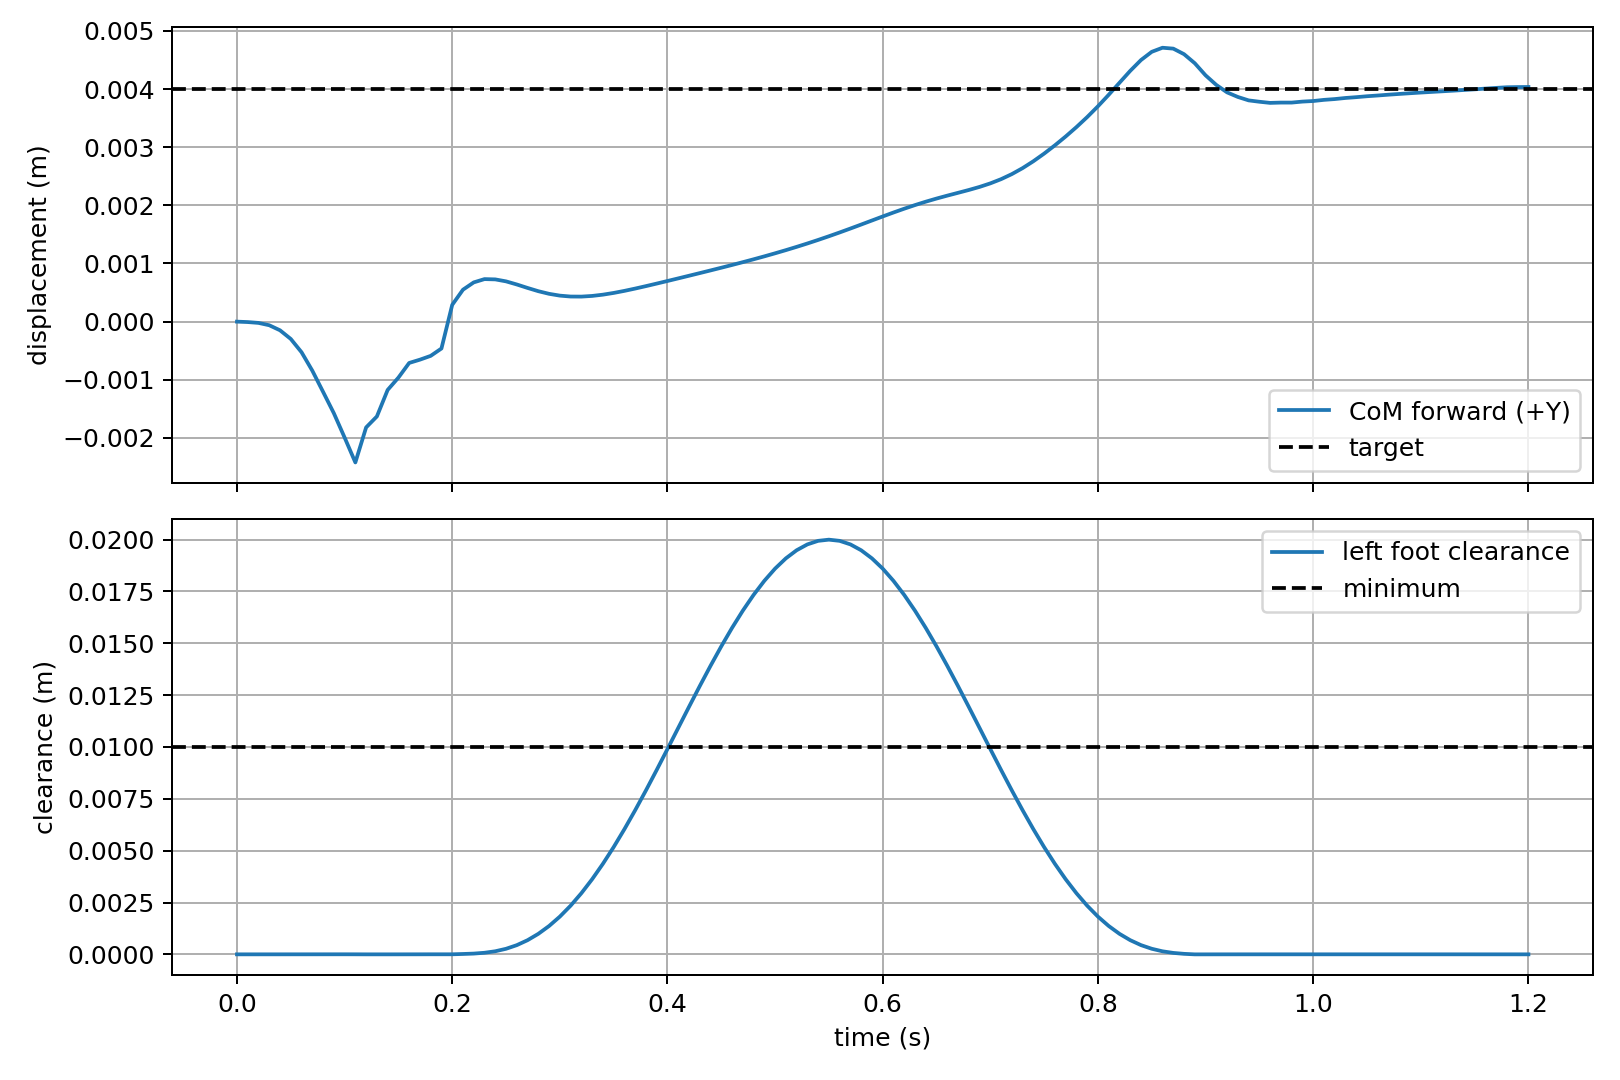
\includegraphics[width=0.48\linewidth]{fddp_single_step_left_swing_com_clearance.png}%
}{\fbox{\parbox[c][3.6cm][c]{0.45\linewidth}{\centering 左脚单步图未随本文件提供}}}%
\hfill
\IfFileExists{fddp_single_step_right_swing_com_clearance.png}{%
  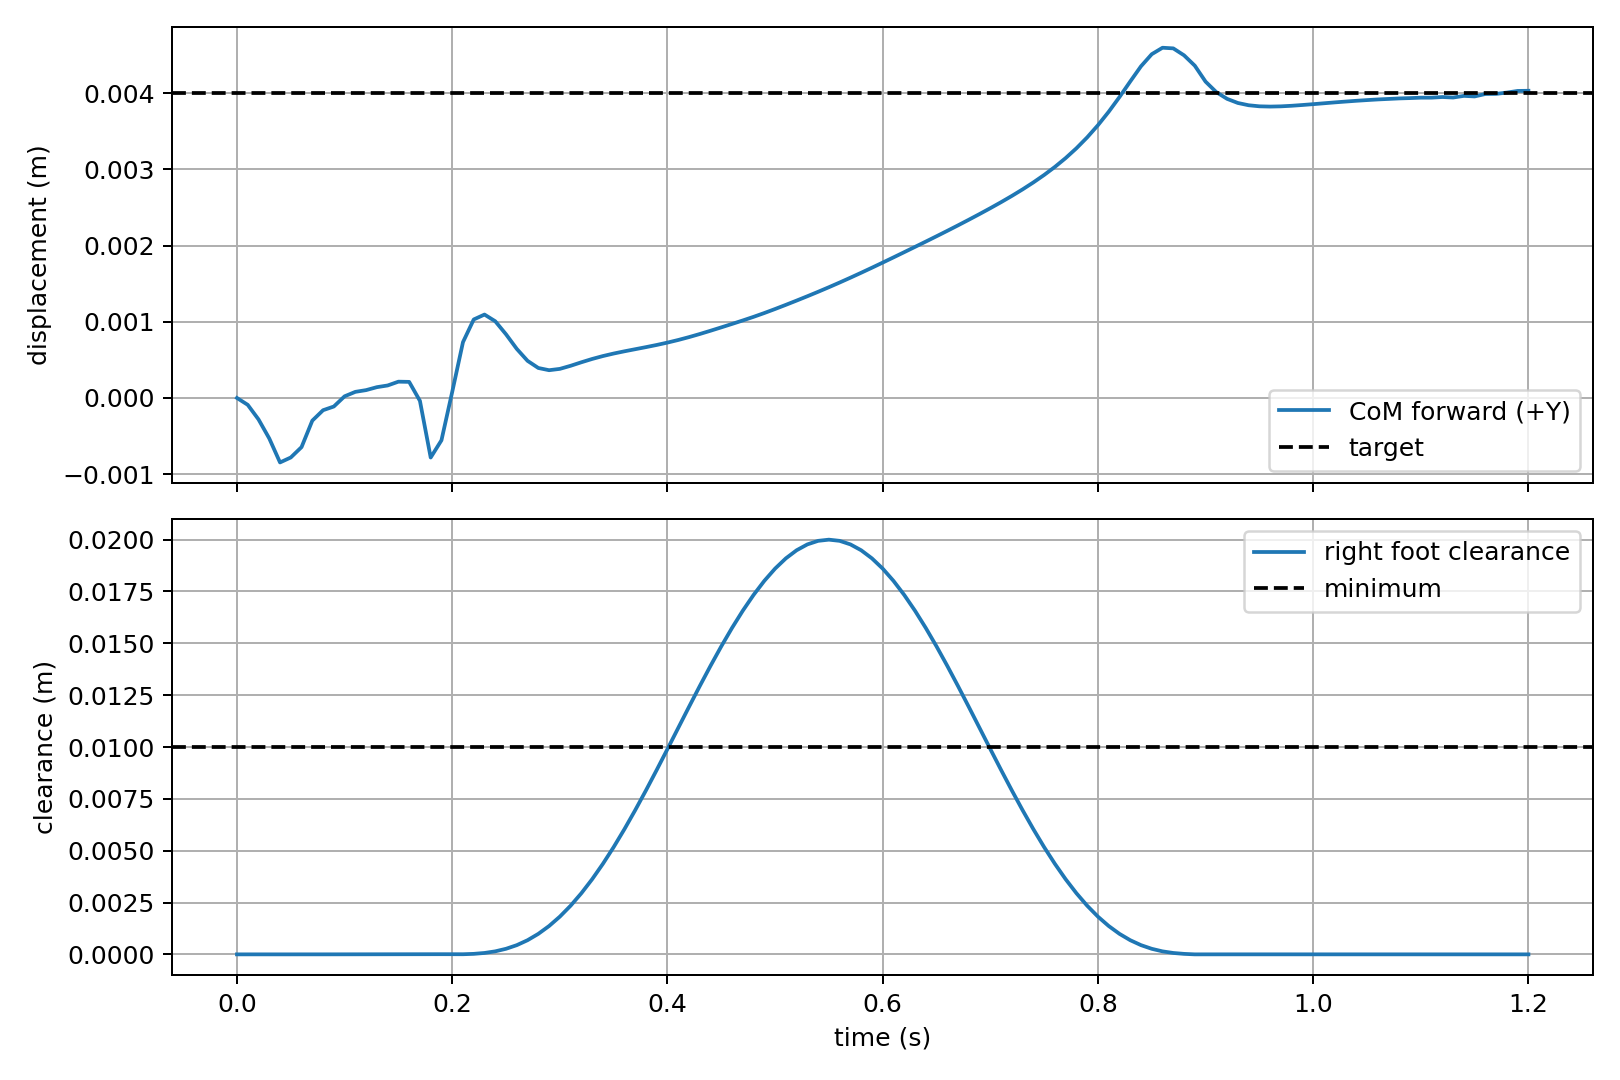
\includegraphics[width=0.48\linewidth]{fddp_single_step_right_swing_com_clearance.png}%
}{\fbox{\parbox[c][3.6cm][c]{0.45\linewidth}{\centering 右脚单步图未随本文件提供}}}
\caption{左右独立 FDDP 单步的 CoM 与 swing clearance。图片为可选资源，缺失时不影响本文档编译。}
\end{figure}

改进 first-order convergence 的优先方法是 continuation/homotopy、合理 scaling、better dynamics-feasible seed、检查 residual derivatives、改变 terminal/control boundary cost，而不是放宽 physical gates。项目后续 periodic cycle 已证明 7-stage homotopy 能把 solver stop 降至 $7.04\times10^{-8}$，说明 continuation 是有依据且在本模型上有效的路线。

\section{从单步到 10-step：证据阶梯与当前边界}\label{sec:multistep}

把“有一条单步轨迹”扩展为“连续稳定行走”至少要跨过四层证据，不能把上一层的通过自动当成下一层通过。

\begin{table}[htbp]
\centering
\caption{FDDP gait 的证据阶梯}
\begin{tabularx}{\linewidth}{@{}p{2.8cm}p{2.2cm}X@{}}
\toprule
层级 & 当前状态 & 含义 \\
\midrule
独立左右单步 & \partialstatus & physical gates 通过，但两个 solver run 均在 500 iterations 后停止，不能称 first-order convergence success \\
两步交替 & \pass & FDDP convergence/gates 与 MuJoCo position-command replay 已完成 \\
Periodic cycle / continuation & \pass & terminal-state 与 boundary-control homotopy 7/7 stages converged \\
10-step planning/contact & \pass & nominal trajectory 与 sagittal contact-feasibility gates 已通过 \\
完整 10-step natural-contact replay & \pass & \SI{10}{s} full replay 通过，20/20 个 liftoff/touchdown 事件按序匹配 \\
FDDP gait batch robustness & \pass & final C2 进行 32 场景 $\times$ 30 seeds，共 960/960 trials 通过 \\
\bottomrule
\end{tabularx}
\end{table}

\subsection{两步与 periodic cycle}

两步交替 FDDP 在 166 iterations 后达到 $\mathrm{stop}=2.84\times10^{-8}$、max shooting gap 0、左右 clearance 约 \SI{20}{mm}、forward CoM \SI{8.118}{mm}，declared trajectory gates passed。MuJoCo position-command replay 的 max joint RMSE 为 $2.707^\circ$，max torso pitch 为 $10.595^\circ$，integrity passed。

periodic two-step cycle 使用 terminal-state 与 boundary-control homotopy；7/7 stages converged，final stop 为 $7.04\times10^{-8}$。它为多步 seed 提供了数值证据，但不是 infinite-horizon limit-cycle proof。

\subsection{10-step planning/contact acceptance}

更新后的 10-step nominal 已通过早期 negative audit 的修复，acceptance state 更新为：
\par\noindent\path{planning_and_contact_accepted}。

\begin{table}[htbp]
\centering
\caption{10-step FDDP nominal 的 planning/contact gates}
\begin{tabular}{@{}lr@{}}
\toprule
Metric & Result \\
\midrule
Solver stop / iterations & $4.4102\times10^{-8}$ / 66 \\
Maximum shooting gap & 0 \\
Maximum active-support translation error & \SI{55.275}{\micro\metre} \\
Maximum landing translation error & \SI{35.726}{\micro\metre} \\
Minimum swing clearance & \SI{19.993}{mm} \\
Minimum joint-limit margin & \SI{11.790}{mrad} \\
Forward CoM displacement & \SI{50.087}{mm} \\
Minimum normal resultant & \SI{9.913}{N} \\
Maximum friction utilisation & 0.5807 \\
Minimum CoP margin & \SI{2.391}{mm} \\
Active contact-row violations & 0 / 1300 \\
\bottomrule
\end{tabular}
\end{table}

\begin{figure}[htbp]
\centering
\IfFileExists{fddp_multistep_contact_feasibility.png}{%
  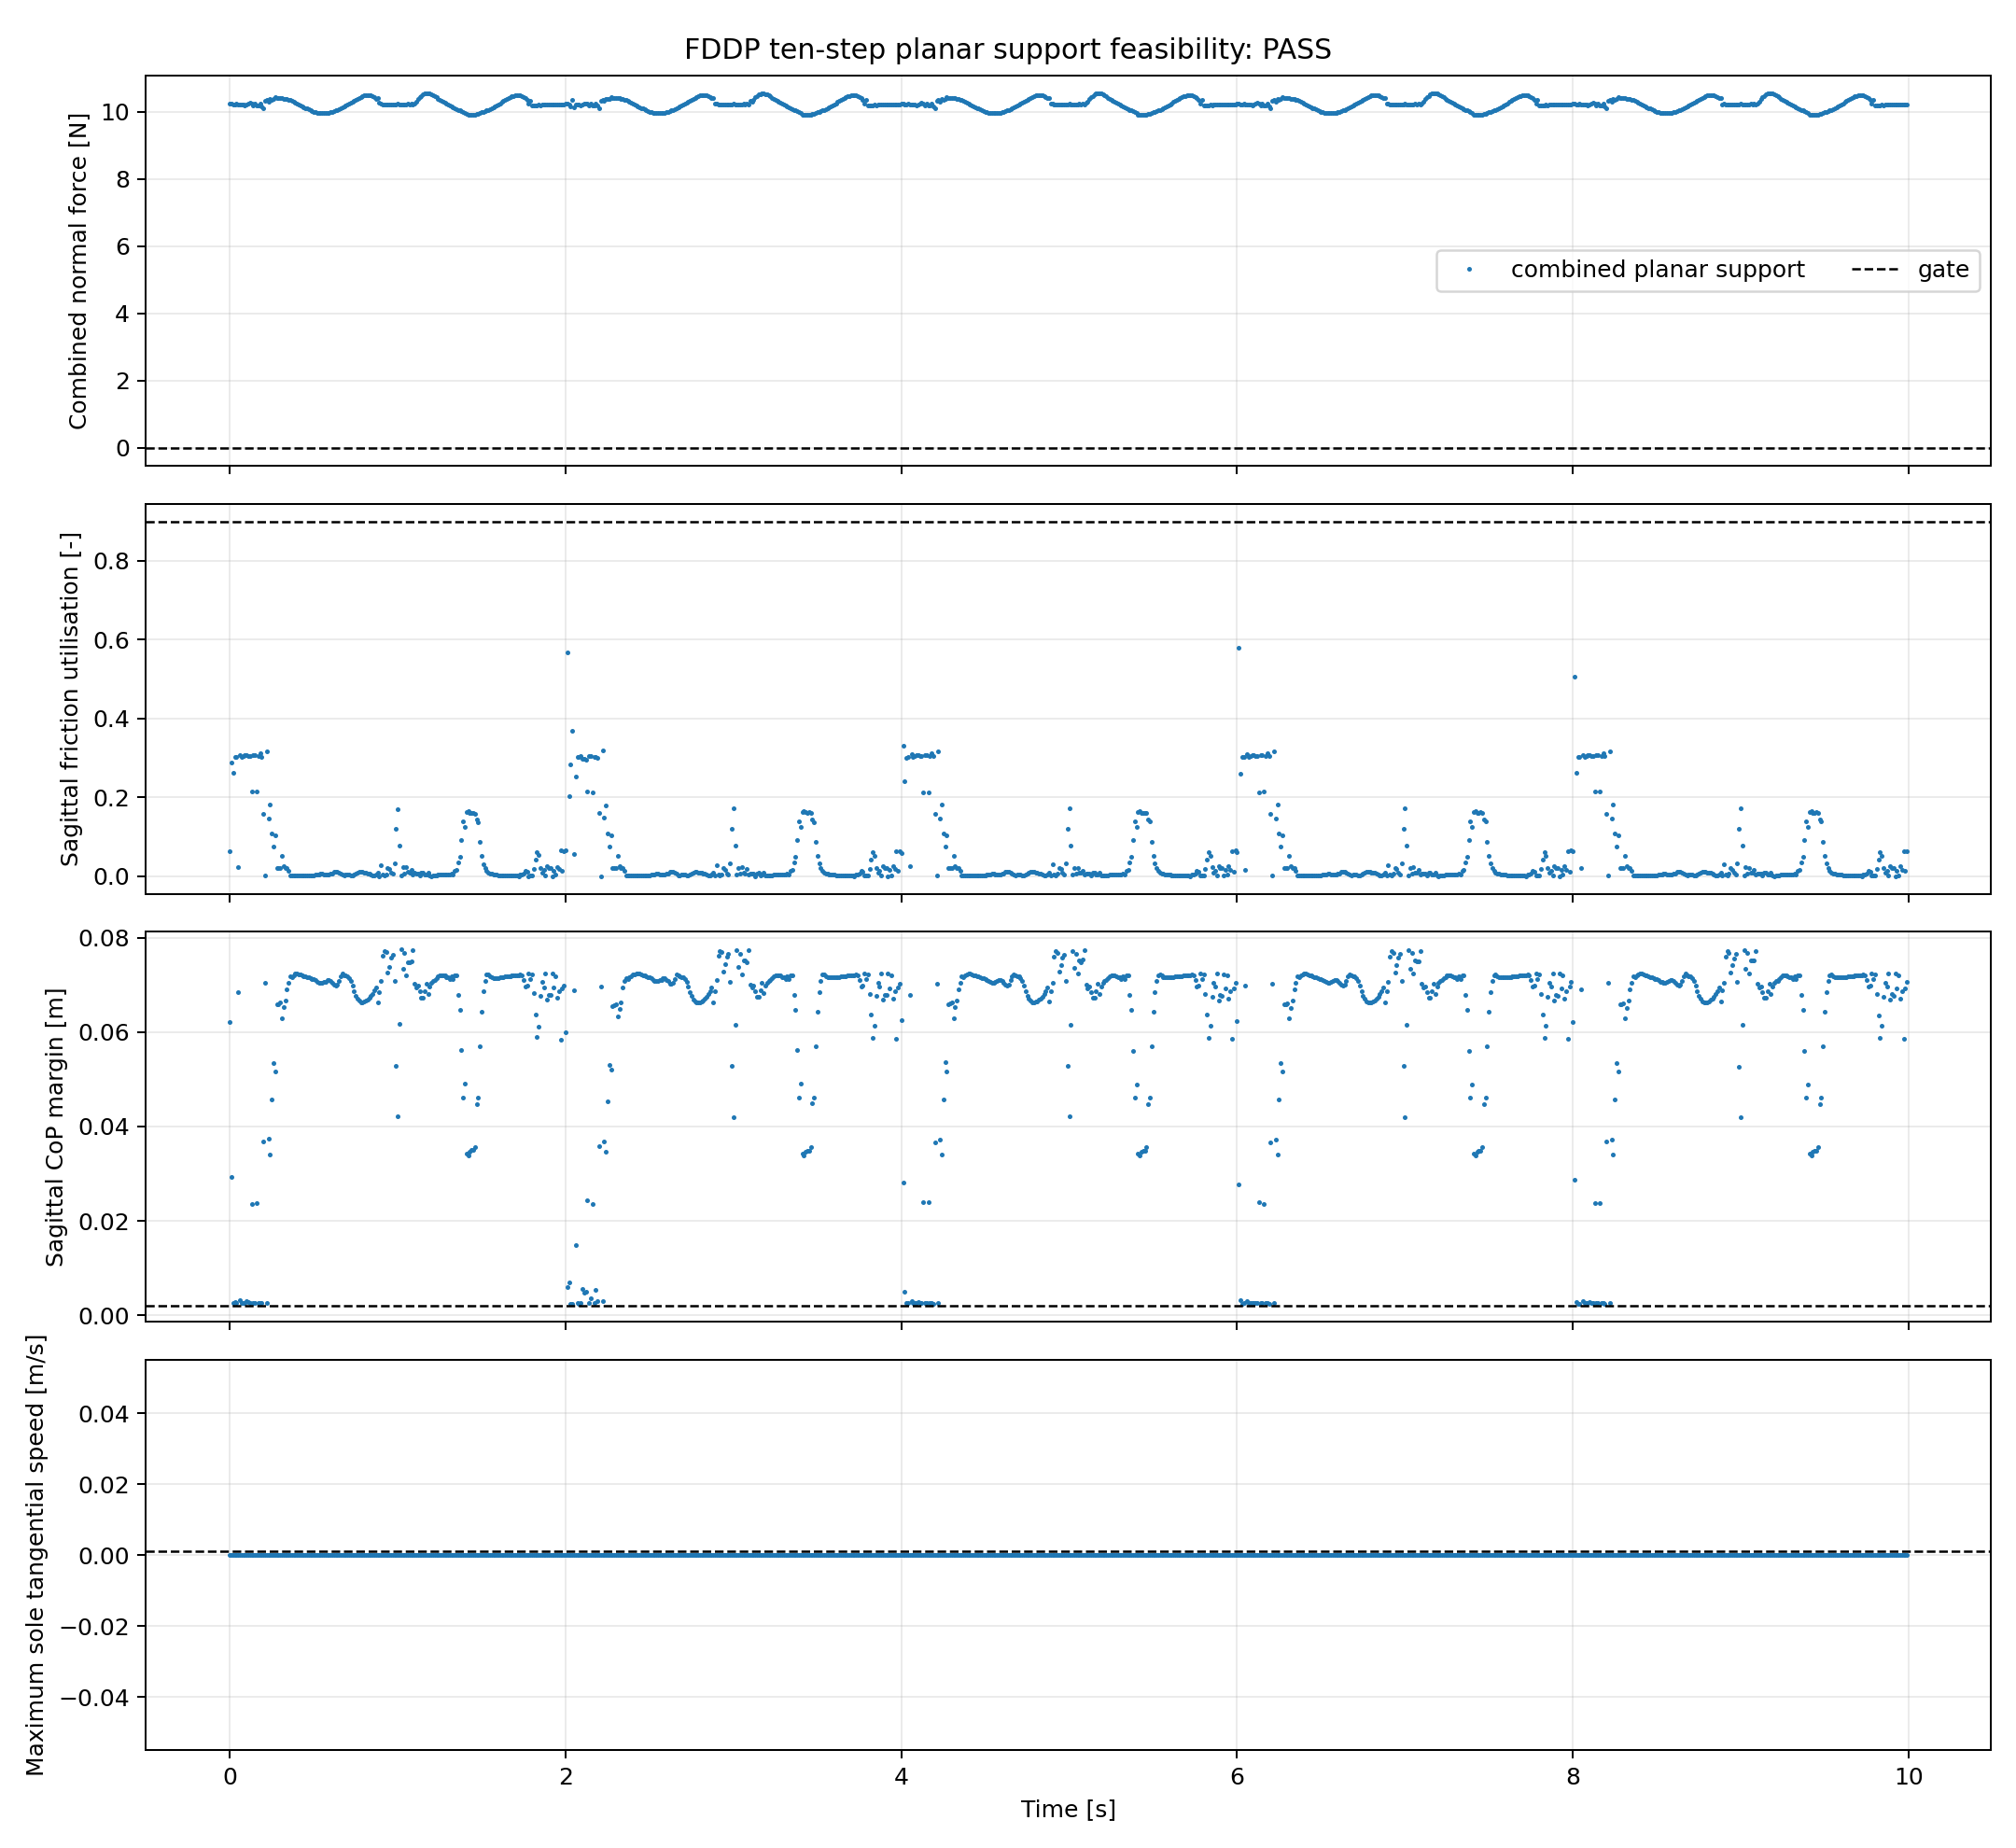
\includegraphics[width=0.90\linewidth]{fddp_multistep_contact_feasibility.png}%
}{\fbox{\parbox[c][4.2cm][c]{0.82\linewidth}{\centering 10-step contact-feasibility figure 未随本文件提供。}}}
\caption{10-step nominal 的 planar-sagittal contact-feasibility audit。通过的是 resultant-level gate；out-of-plane 分量仅作模型诊断，DS per-foot load split 不作唯一物理解读。}
\end{figure}

旧记录中的 75 个 violation、friction utilisation 2.165 和 CoP margin $-416.6$ mm 是修复前的历史结果，应保留在实验演进记录中，但不能继续写成当前结论。

\section{MuJoCo position-command replay：验证什么、当前结果是什么}\label{sec:replay}

Replay 读取 $q_{\mathrm{ref}}$，经过 delay、first-order lag 与 speed-limit actuator proxy，再交给 MJCF position actuators；它不把 $\tau_{\mathrm{ref}}$ 当作 actuator command。它用于测量 planner model、simulator model 与 position-command path 之间的 mismatch。

正式 10-step nominal replay 已覆盖完整 \SI{10}{s}：simulation finite、无 fall，maximum joint RMSE 为 $1.124^\circ$，maximum absolute torso pitch 为 $9.479^\circ$，minimum torso-height fraction 为 0.9789，无 unintended flight、无 sustained penetration。20 个 scheduled left/right liftoff/touchdown events 全部按序匹配，event match ratio 为 1.0，replay acceptance 与 integrity 均为 true。执行层使用经过验收的 \SI{30}{ms} command-reference advance 补偿 position-actuator delay；该值属于本模型/执行器代理的标定量，不应写成普适常数。

\begin{figure}[htbp]
\centering
\IfFileExists{fddp_multistep_nominal_replay.png}{%
  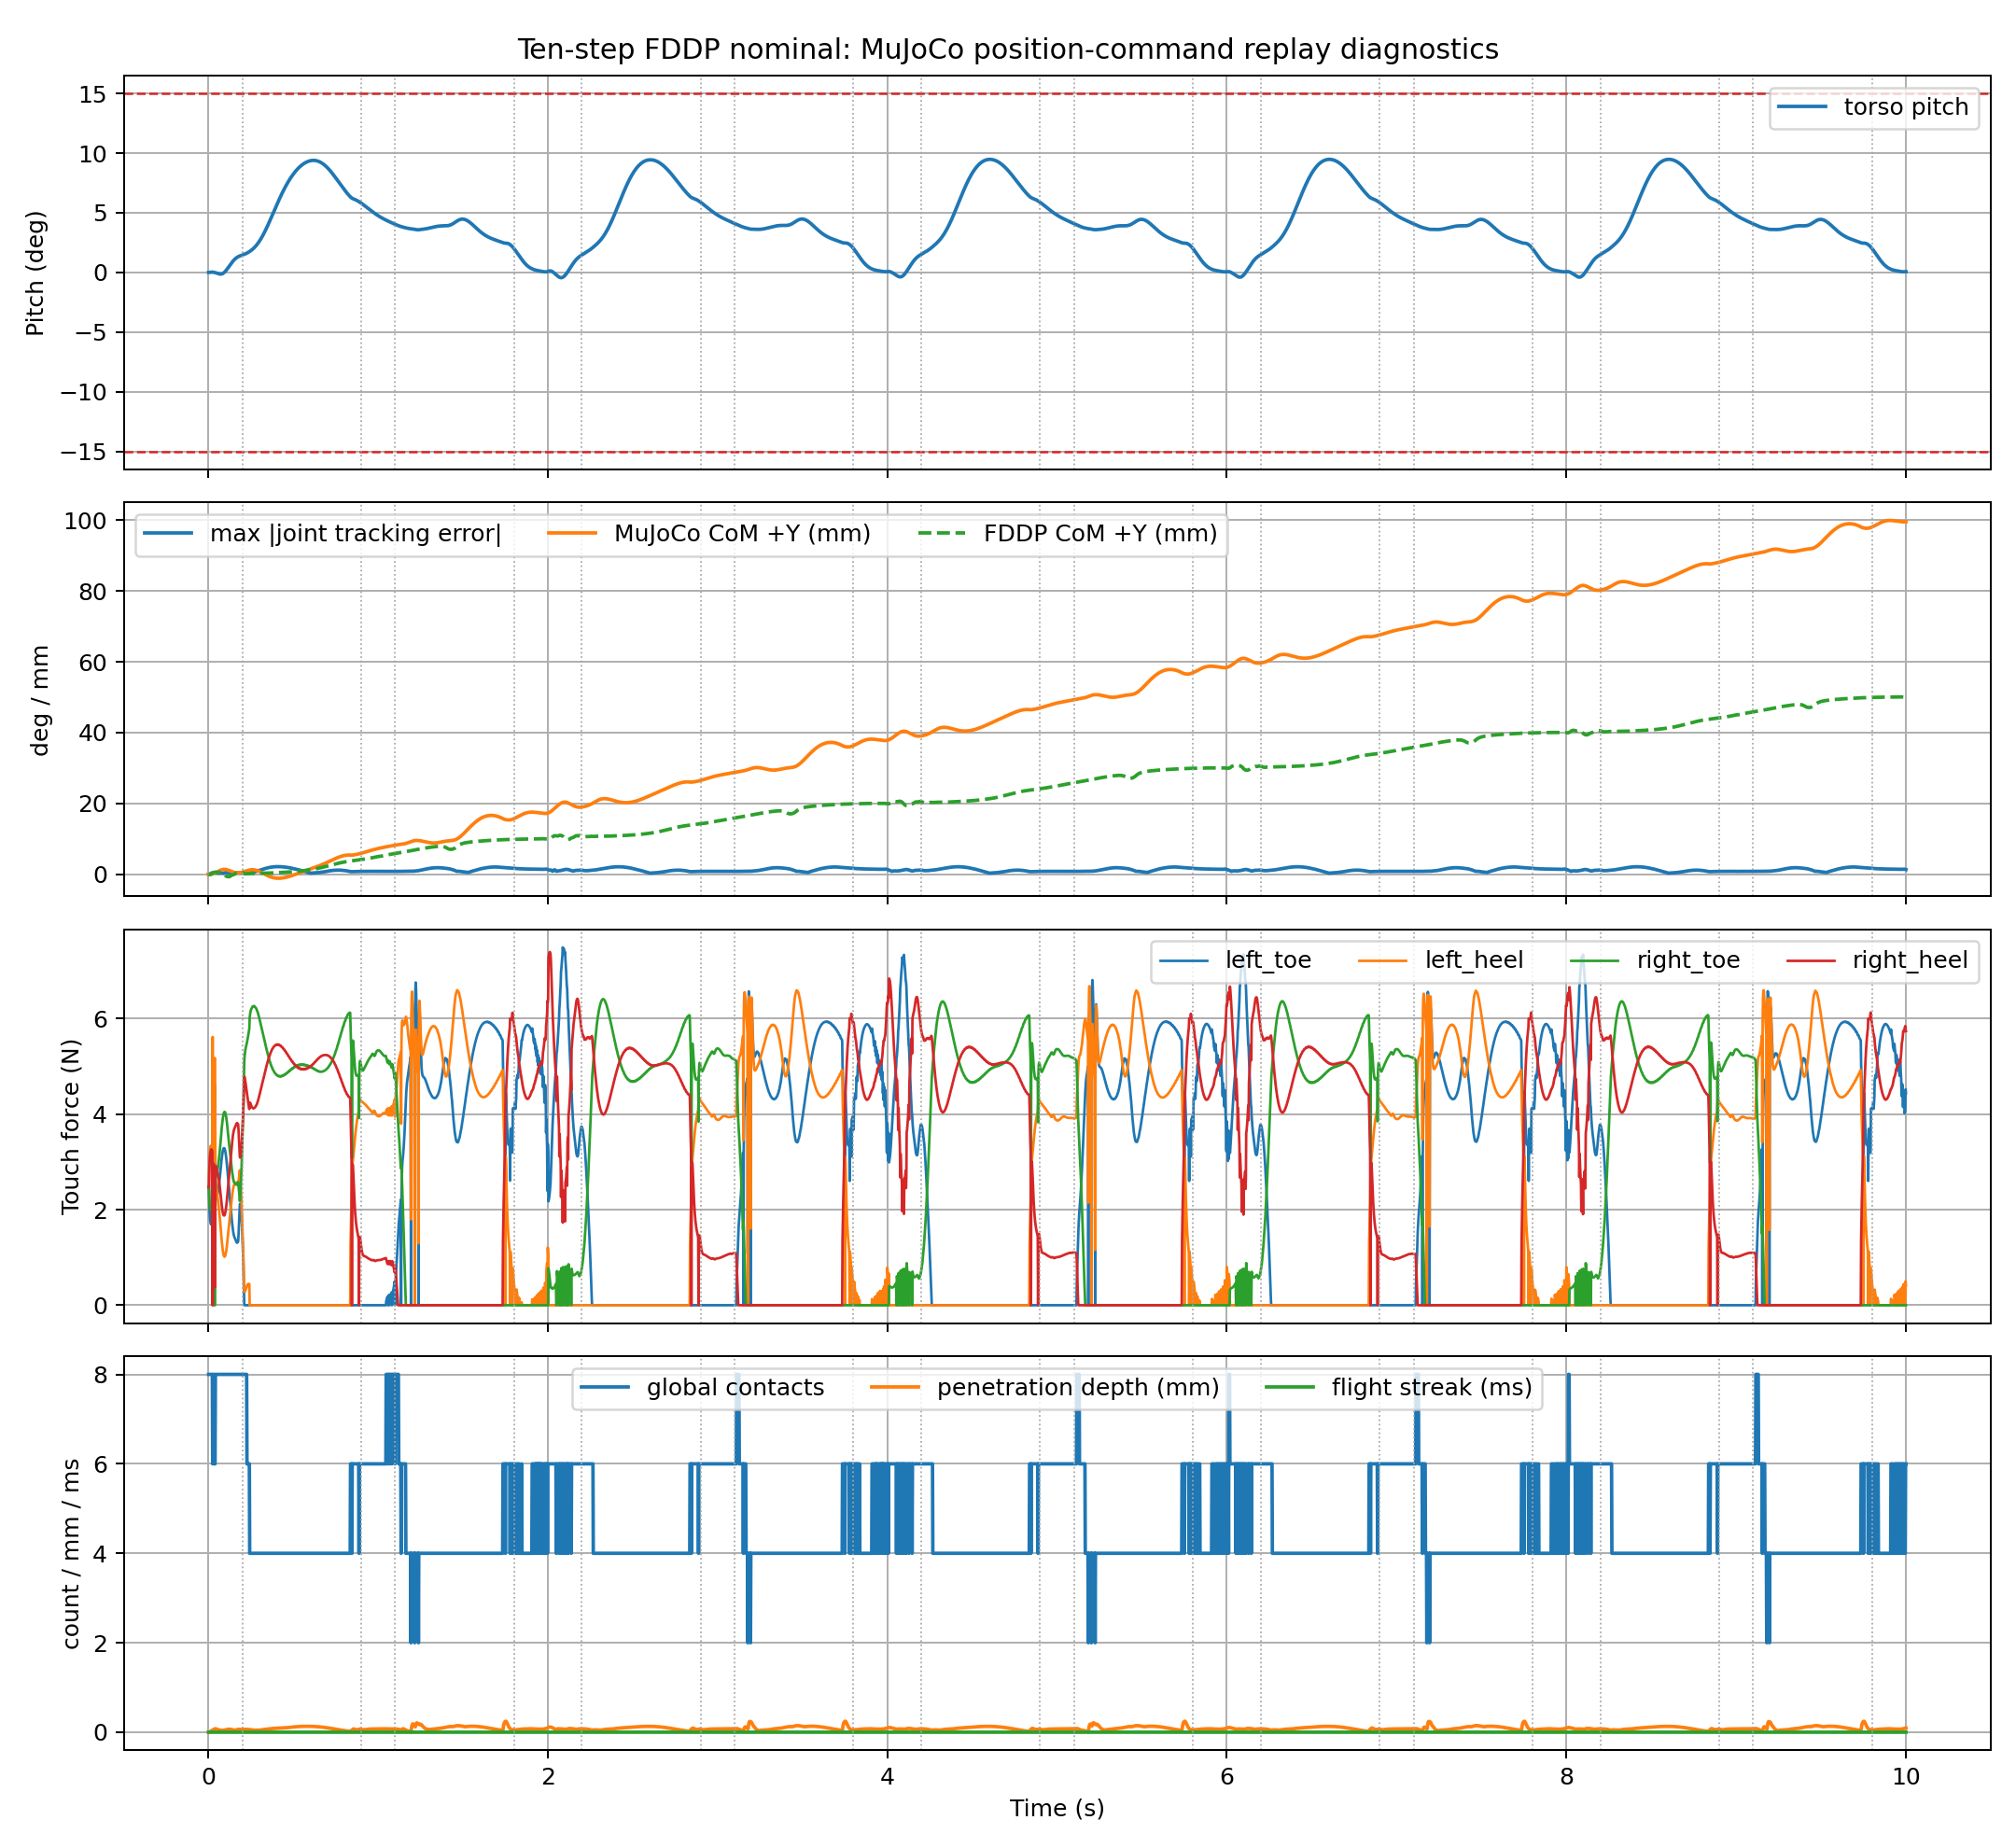
\includegraphics[width=0.90\linewidth]{fddp_multistep_nominal_replay.png}%
}{\fbox{\parbox[c][4.2cm][c]{0.82\linewidth}{\centering full 10-step replay figure 未随本文件提供。}}}
\caption{完整 10-step MuJoCo nominal replay。图中应同时阅读 joint tracking、torso pitch、height 与逐脚 contact events，不能只凭动画判断成功。}
\end{figure}

因此当前结论是：\textbf{10-step planning/contact accepted，full natural-contact replay accepted}。这一结论由 20/20 逐脚 event audit、position tracking、pitch、height、flight 与 penetration gates 共同支持，而不是只由 \code{min global contact count} 支持。

\section{C0、C1 与 C2：三个 controller 怎样逐层增加能力}\label{sec:c012}

三个 controller 不是三套互相竞争的完整 walking controller，而是同一 position-command pipeline 的增量实验层。

\begin{longtable}{@{}p{0.10\linewidth}p{0.31\linewidth}p{0.47\linewidth}@{}}
\toprule
层级 & Command / mechanism & 回答的问题 \\
\midrule
\endhead
C0 & $\bm q_{\mathrm{cmd}}=\bm q_{\mathrm{ref}}$ & 无 online correction 时 nominal replay 的基线表现。\\
C1 & $\bm q_{\mathrm{cmd}}=\bm q_{\mathrm{ref}}+\bm G\alpha$ & reference clock 固定时，FIR-QP-MPC 能否改善 torso-pitch recovery。\\
C2 & C1 command path + event-based reference retiming & observed liftoff/touchdown 与 schedule 不一致时，怎样调整读取 $\bm q_{\mathrm{ref}}$ 的 phase。\\
\bottomrule
\end{longtable}

\subsection{Fixed mapping：为什么 QP 只优化一个变量}\label{sec:mapping}

C1 优化 scalar $\alpha$，再通过
\begin{equation}
 \Delta\bm q=\bm G\alpha,\qquad
 \bm G=[0.27,\,0.062,\,-0.228,\,0.27,\,0.062,\,-0.228]^{\mathsf T}
\end{equation}
分配到六个关节。这样把 online decision dimension 从六维 joint correction 降为一个协调模式：可以用 calibration pulse 直接辨识 $\alpha\rightarrow$ pitch response，QP 规模也很小。该 mapping 是当前 operating region 中的经验 control direction，不是普遍最优 whole-body feedback；contact mode、姿态或 disturbance 类型改变时应重新辨识，或扩展为多个 basis vectors。

\subsection{FIR、AR 与 prediction model}\label{sec:firqp}

FIR（Finite Impulse Response）用有限历史描述 correction 到 pitch output 的 delayed response：
\begin{equation}
 \hat y_k=\sum_{i=0}^{M-1}h_i\alpha_{k-i}.
\end{equation}
最终 10-step identification 使用 pulse width \SI{20}{ms}、sample period \SI{20}{ms}，导出 $M=23$ 个 FIR coefficients，与 \SI{50}{Hz} controller period 对齐。FIR 的优点是结构简单、因果、计算量固定；缺点是只能在辨识过的局部幅值和接触条件附近可靠。

AR term 用近期输出误差描述未被 FIR 输入通道解释的自然衰减或振荡。可以把 free response 写成
\begin{equation}
 \hat e_{k+1}^{\mathrm{free}}=\sum_{j=0}^{p-1}a_j e_{k-j}.
\end{equation}
项目中的 FIR 与 AR 不是两个独立 controller：AR 估计没有新 correction 时误差怎样发展，FIR 估计候选 correction 会增加怎样的响应，两者共同形成 QP prediction。

\subsection{QP objective 与约束}

在 prediction horizon $N=12$ 内构造 dynamic matrix $\bm S$，求解
\begin{equation}
 \min_{\bm\alpha}\;
 q\lVert\bm e_{\mathrm{free}}+\bm S\bm\alpha\rVert_2^2
 +r\lVert\bm\alpha\rVert_2^2
 +s\lVert\bm D\bm\alpha-\bm d_{\mathrm{prev}}\rVert_2^2,
 \label{eq:qp}
\end{equation}
并施加 amplitude 与 slew-rate box constraints。第一项抑制 predicted pitch error，第二项避免过大 correction，第三项抑制命令突变。receding horizon 只执行第一步，然后用新观测重算。

\subsection{C1 parameter evidence：historical balanced 与 final r\_low}\label{sec:balanced}

\begin{table}[htbp]
\centering
\caption{历史 balanced candidate 在 CoM-shift replay 上的 holdout result}
\begin{tabular}{@{}lrrr@{}}
\toprule
Direction & Pitch IAE: C0 $\rightarrow$ C1 & Reduction & Settling: C0 $\rightarrow$ C1 \\
\midrule
Forward & $0.2710\rightarrow0.2474$ & 8.7\% & $\SI{0.248}{s}\rightarrow\SI{0.166}{s}$ \\
Backward & $0.2681\rightarrow0.2295$ & 14.4\% & $\SI{0.246}{s}\rightarrow\SI{0.166}{s}$ \\
\bottomrule
\end{tabular}
\end{table}

maximum correction 分别为 $0.711^\circ$ 和 $0.669^\circ$。这组 balanced result 是历史 CoM-shift holdout 证据。最终 10-step common-protocol experiment 重新复用 one-factor candidates；在 \SI{20}{ms} FIR 对齐后，\code{r\_low}（$q=1500,r=10,s=25$）使 C1 IAE 从 3.7588 降到 3.3534 deg\,s，即改善 10.79\%，同时 peak 从 $1.990^\circ$ 降到 $1.822^\circ$。因此论文应把 balanced 写成 earlier local evidence，把 \code{r\_low} 写成 final 10-step selection，不能混成同一个结果。

holdout validation 表示参数选择与最终评估使用不同 disturbance cases，降低“在同一组数据上调参再宣布成功”的风险。它增强 generalisation evidence，但不等于覆盖所有步态相位、地形与执行器误差。

\begin{figure}[htbp]
\centering
\IfFileExists{c1_qp2_forward_pitch_comparison.png}{%
 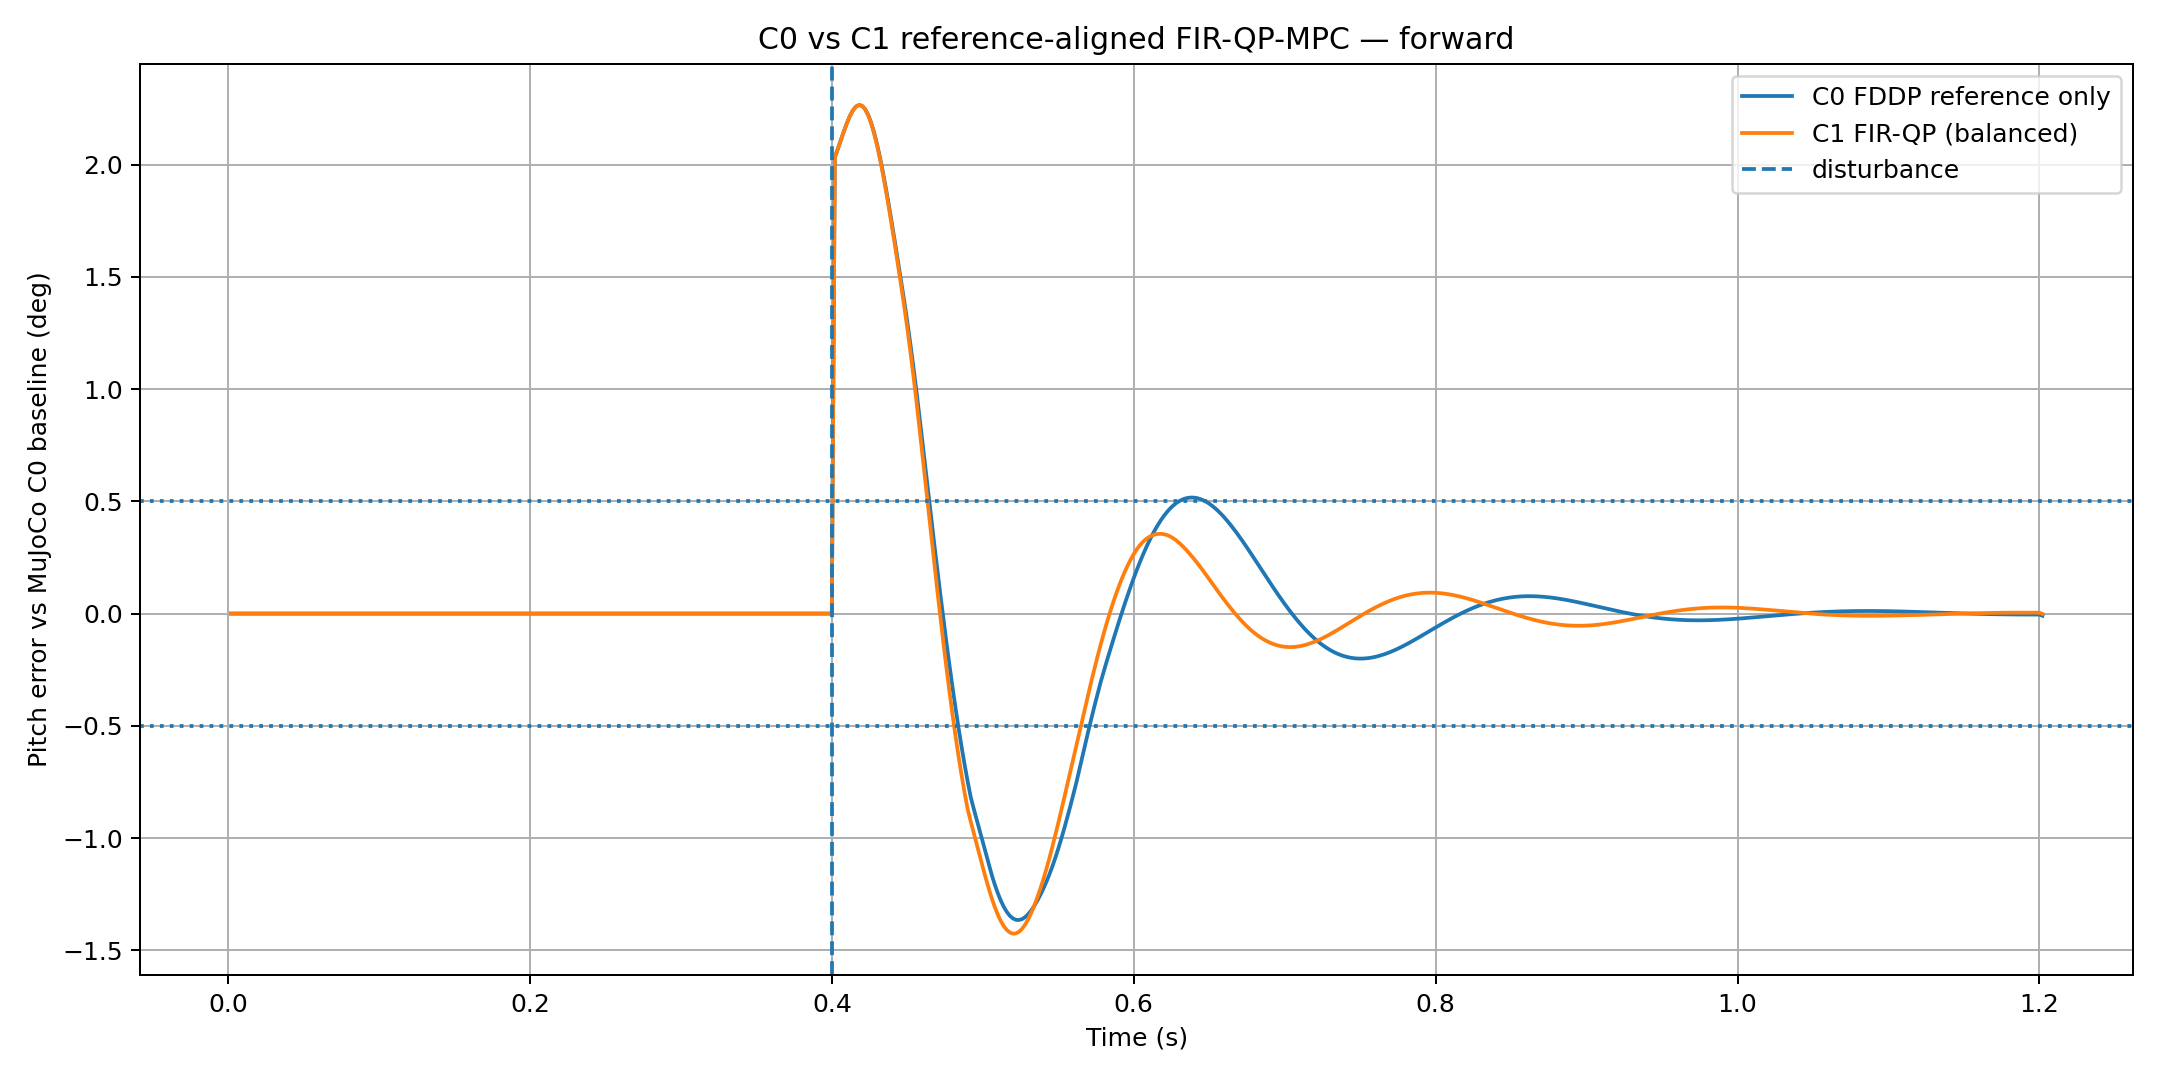
\includegraphics[width=0.88\linewidth]{c1_qp2_forward_pitch_comparison.png}%
}{\fbox{\parbox[c][4.0cm][c]{0.80\linewidth}{\centering C1 forward pitch comparison figure 未随本文件提供。}}}
\caption{C0 与 C1 的 forward disturbance recovery comparison。解读重点是 IAE、settling time 与 correction magnitude，而不是只看单个峰值。}
\end{figure}

\subsection{C2-final：按事件类型的局部腿 phase synchronisation}\label{sec:c2}

MuJoCo toe/heel normal force 先经 threshold 与 debounce 形成 foot-contact Boolean；当前 threshold 为 \SI{0.25}{N}，debounce 为 \SI{10}{ms}。完整 10-step replay 显示的主要 mismatch 不是“所有事件统一偏移”：liftoff 通常比 schedule 晚约 \SI{110}{ms}，而 touchdown 基本准时。因此单一 global offset 会让准时 touchdown 抵消 late liftoff correction，甚至把整机 nominal phase 一起移动而增加 torso-pitch error。

最终 C2 使用 \textbf{event-type memory + local-leg retiming}。对每一种 left/right liftoff/touchdown 分别保存 bounded predictive offset：
\begin{equation}
 \delta t_j^{+}=\operatorname{clip}\!\left[
 \delta t_j+\gamma\left(e_{t,j}-\delta t_j\right),
 -\delta t_{\max},\delta t_{\max}\right],
 \qquad
 e_{t,j}=t_{\mathrm{obs},j}-t_{\mathrm{expected},j}.
\end{equation}
当前实例使用 $\delta t_{\max}=\SI{100}{ms}$、maximum update step \SI{40}{ms}、$\gamma=0.75$。fixed wall-time clock 继续提供 torso-pitch baseline 与支撑腿 nominal；motion clock 只替换“下一 contact event 所属腿”的三个 joint references。这样 phase synchronisation 改善 physical contact timing，同时避免把整机 pitch baseline 一起平移。

最终 command path 还包含三个容易在论文中遗漏、但对结果关键的工程处理：
\begin{enumerate}
 \item \SI{30}{ms} command-reference advance 补偿 position-actuator delay；
 \item SafetyLimiter 采用 reference-relative update，只限制 $\Delta\bm q$ 的变化并继续检查 absolute joint limits，不再拖慢完整 $\bm q_{\mathrm{ref}}$；
 \item FIR pulse width 与 sampling period 均与 controller 的 \SI{20}{ms} 周期对齐；最终复用 one-factor ablation 中的 \code{r\_low} candidate，即 $q=1500,r=10,s=25$。
\end{enumerate}

\begin{table}[htbp]
\centering
\caption{完整 10-step 同协议 C0/C1/phase-only/C2-final 消融}
\begin{tabular}{@{}lrrrr@{}}
\toprule
Mode & Peak pitch error & IAE & Mean contact error & Event match \\
\midrule
C0 & $1.990^\circ$ & 3.7588 deg\,s & \SI{56.7}{ms} & 20/20 \\
C1 & $1.822^\circ$ & 3.3534 deg\,s & \SI{56.6}{ms} & 20/20 \\
phase-only & $1.990^\circ$ & 3.5760 deg\,s & \SI{30.9}{ms} & 20/20 \\
C2-final & $1.822^\circ$ & 3.3202 deg\,s & \SI{35.0}{ms} & 20/20 \\
\bottomrule
\end{tabular}
\end{table}

在相同 \SI{2}{\degree} pitch 和 \SI{0.25}{rad/s} disturbance 下，C1 IAE 相对 C0 改善 10.79\%；C2-final 的 IAE 进一步优于 C1，peak 不增加；C2-final contact timing error 相对 fixed-phase C1 改善 38.16\%。五项 acceptance checks 全部通过，20/20 events 有序匹配，limiter/saturation fraction 均为 0。可复核来源是 \path{results/logs/fddp_multistep_controller_ablation.yaml}，不是旧的 two-step C2 局部结果。

\begin{figure}[htbp]
\centering
\IfFileExists{fddp_multistep_controller_ablation.png}{%
 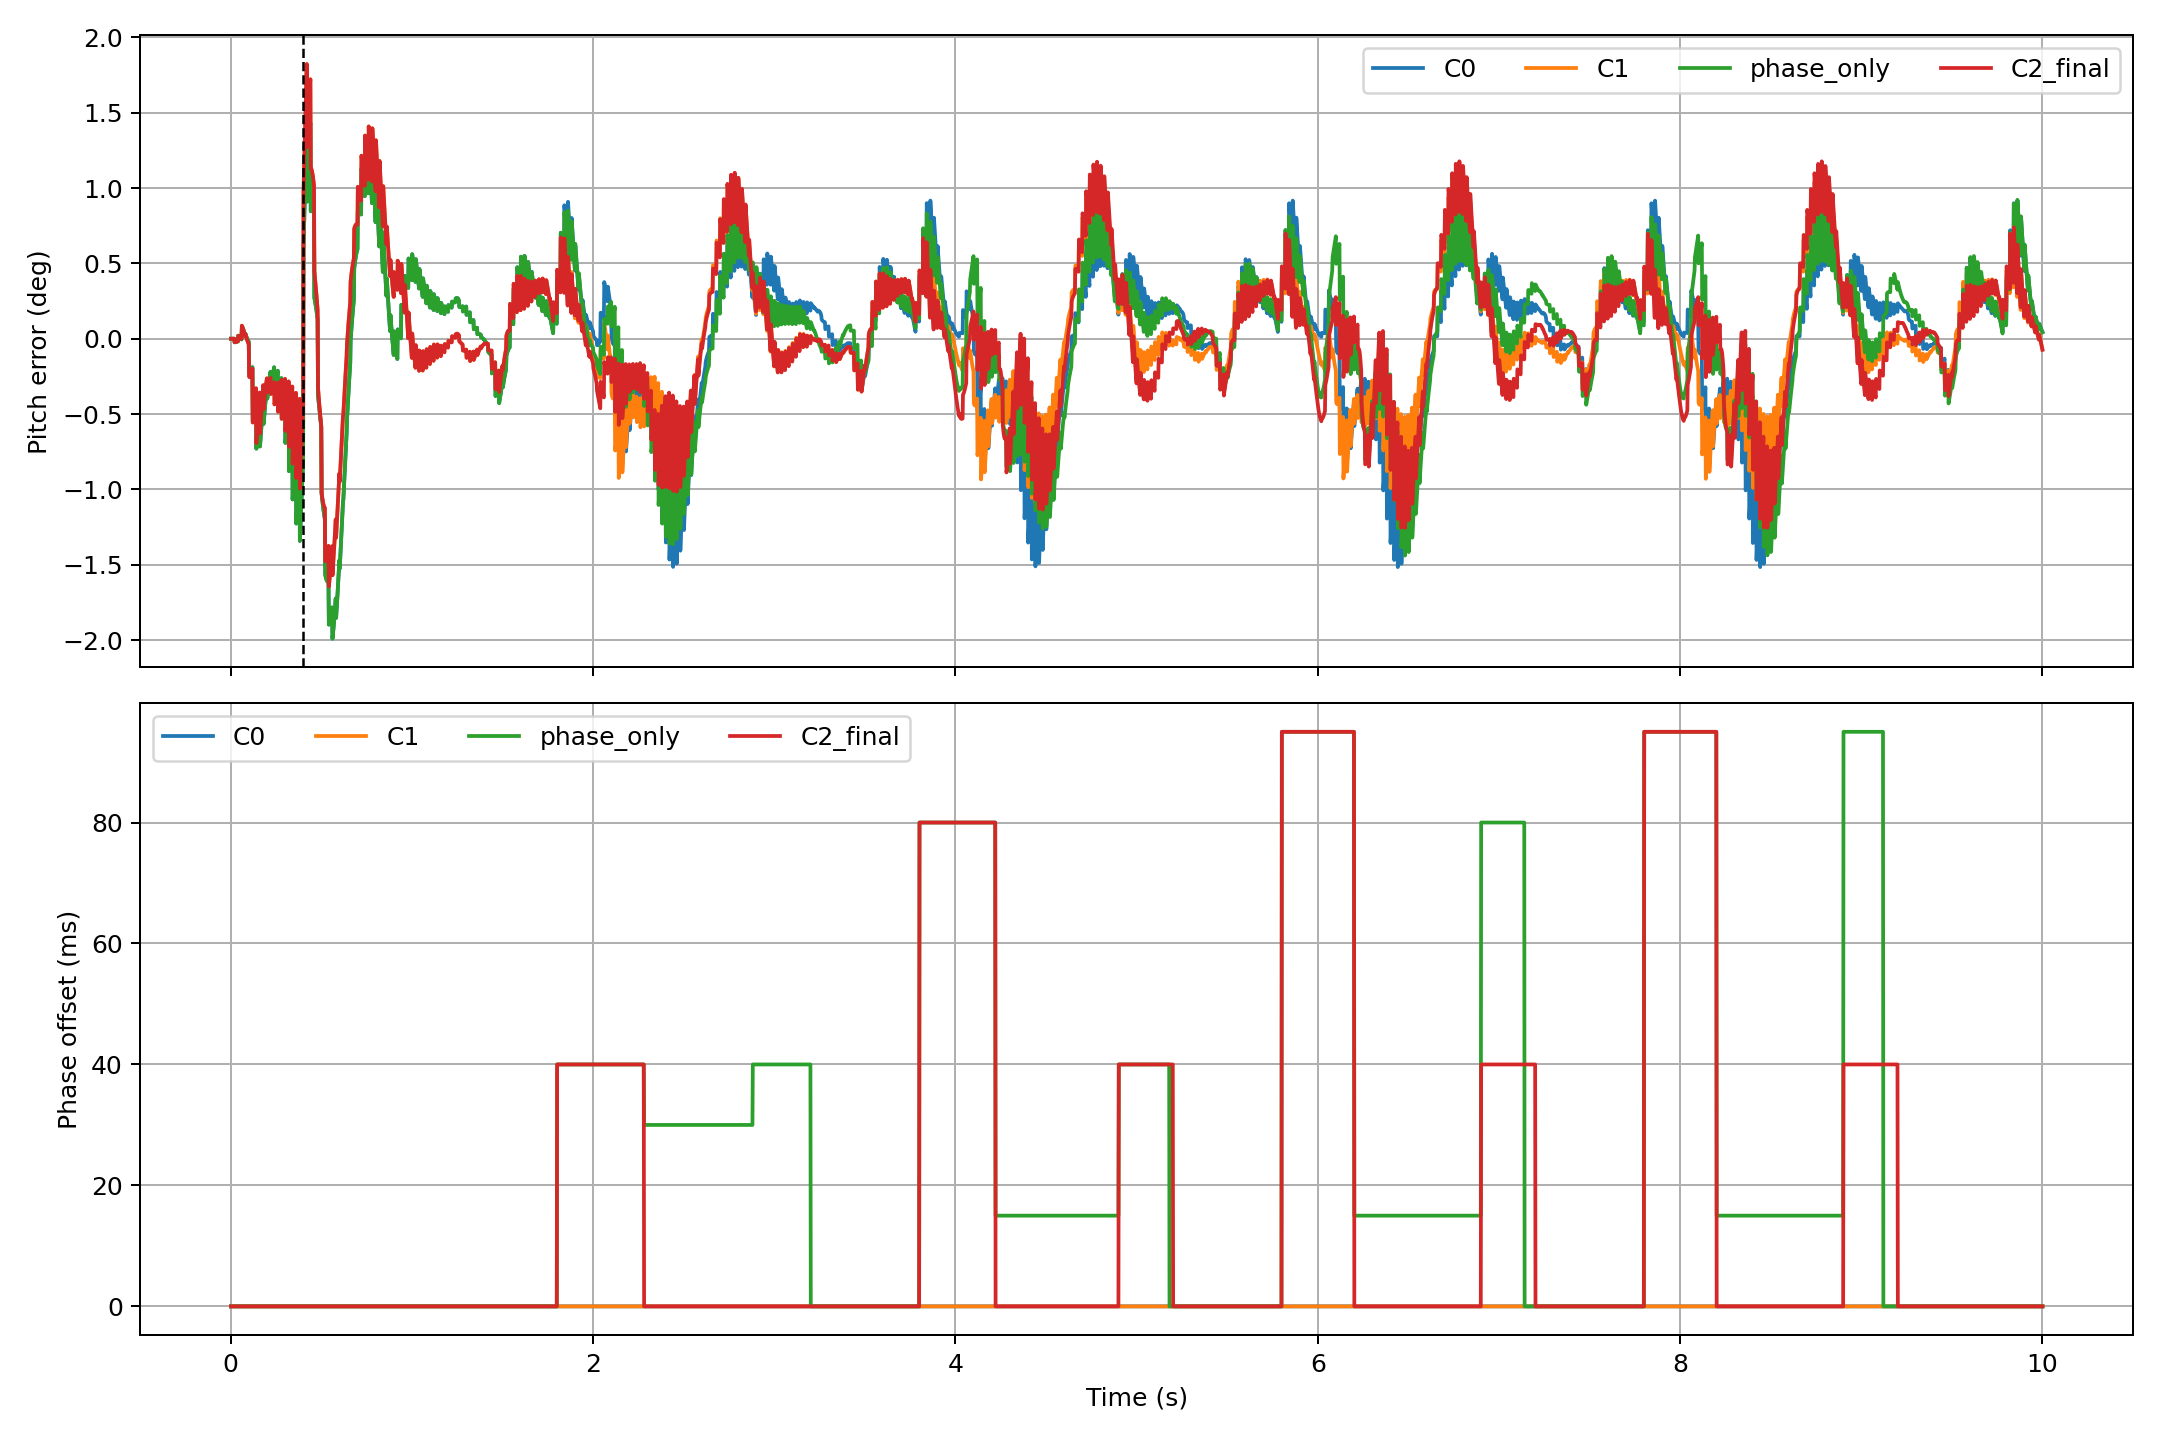
\includegraphics[width=0.92\linewidth]{fddp_multistep_controller_ablation.png}%
}{\fbox{\parbox[c][4.0cm][c]{0.84\linewidth}{\centering 10-step controller ablation figure 未随本文件提供。}}}
\caption{C0/C1/phase-only/C2-final 的 common-protocol pitch-error 与 phase-offset comparison。论文正文应配合表格报告 acceptance thresholds，不能只展示曲线。}
\end{figure}

\section{E1--E6：证据怎样组织}\label{sec:evidence}

\begin{longtable}{@{}p{0.09\linewidth}p{0.29\linewidth}p{0.48\linewidth}@{}}
\toprule
编号 & 验证主题 & 可复核证据 \\
\midrule
\endhead
E1 & FDDP convergence/feasibility & iteration cost、solver stop、shooting gap、derivative audit、contact/joint/CoM gates。\\
E2 & C0 nominal replay & 无 online correction 的 joint tracking、pitch、height、contacts 与 CoM baseline。\\
E3 & C1 correction & 同一 disturbance 下 C0/C1 的 IAE、settling、peak 与 correction magnitude。\\
E4 & FIR holdout & 未参与 identification 的 pulse polarity/case 上的 prediction performance。\\
E5 & contact-timing mismatch & early/late touchdown、delay、brief contact loss 下的 event match 与 phase offset。\\
E6 & timing/safety & controller runtime 相对 deadline，并显式报告 limiter、fallback 与 fault handling 是否存在。\\
\bottomrule
\end{longtable}

E1--E6 是 evidence organisation，不是六个 controller。每个 thesis claim 必须能回到 YAML 与 CSV、figure、command 和 interpreter。
GIF 只能帮助观察，不能代替数值 gate。

\section{Robustness matrix：怎样证明不是“碰巧跑通”}\label{sec:robustness}

\subsection{先解释 trial、seed、scenario 和 gate}

\begin{intuitionbox}
一次仿真叫一个 \textbf{trial}；一种测试条件叫一个 \textbf{scenario}；\textbf{seed} 是伪随机数种子，让噪声或初值变化可以重复；\textbf{gate} 是预先写好的及格线。批量测试的目的不是制造更多曲线，而是避免只挑最好的一次展示。
\end{intuitionbox}

若某场景运行 $n$ 次、通过 $k$ 次，样本成功率为
\begin{equation}
 \hat p=\frac{k}{n}.
\end{equation}
Wilson confidence interval 用于提醒读者“小样本全过”仍有很大不确定性。例如历史 scripted gait 中的 5/5，其 95\% Wilson lower bound 仅约 0.566；即使 5 次全过，也不能写成总体成功率接近 100\%。当前 960/960 若形式上按独立同分布 trial 计算，aggregate lower bound 约为 0.996，但这些 trial 来自结构化仿真场景，仍不能外推为任意环境或硬件成功率。

\subsection{历史负结果怎样推动设计修改}

早期 Stage 8/9 使用人工 scripted alternating reference，共 70 trials；强 forward push $+\SI{4}{N}$ 时 C0 与当时的 C2 都是 0/5。这个结果没有被删除，因为它说明旧配置没有恢复能力，也促使后续把测试迁移到 accepted 10-step FDDP nominal，并重新调整 FIR recovery response。历史 70-trial 结果只证明旧 scripted pipeline 的表现，不是当前 final FDDP gait 的结论。

\subsection{第一层：双方向强推恢复}

在相同的 \SI{10}{s} position-command simulation 中，于 \SI{0.8}{s} 施加持续 \SI{0.12}{s} 的 $\pm\SI{4}{N}$ push。候选 \code{fir\_fast} 被选中，forward 为 30/30，backward 为 30/30，达到预先设定的至少 90\% 成功率门槛。因为这一阶段已通过，phase gain scheduling 与 bounded foothold 分支没有继续执行；尤其不能声称“在线落脚点优化已完成”，因为改变 foothold 需要重新生成 reference 并重新做 contact-feasibility gate。

\subsection{第二层：15 类 fault injection}

故障注入不是模拟“机器人一定不会摔”，而是故意提供坏输入，检查程序会不会输出 NaN、越过关节限位或直接崩溃。当前 15 类场景覆盖 stale/NaN/Inf pitch、接触传感器 stuck、事件丢失/乱序、invalid QP、deadline miss、命令/速率饱和、执行器延迟和 reference 缺失/截断/schema 错误。全部场景均被接受，未捕获异常为 0，命令保持 finite、within limits 且 rate-bounded。

安全状态的直观含义为：\code{NORMAL} 正常运行；\code{DEGRADED} 暂时降低功能；\code{FALLBACK} 回到 C0 nominal；\code{SAFE\_HOLD} 保持安全姿态命令；\code{FAILED} 在启动前拒绝无效 reference。它证明的是 software fault containment，不是经过真实传感器、电机和通信链验证的 functional safety certification。

\subsection{第三层：final FDDP-gait statistical robustness}

正式矩阵运行 final C2 position-command pipeline：32 个场景，每个 30 seeds，共 960 trials。场景覆盖 nominal、$\pm2/\pm4$ N push、摩擦、$\pm3/\pm5^\circ$ 坡度、2/4/6 mm 台阶、command/sensor delay、actuator gain/time constant、initial joint/pitch noise 和 combined cases。结果为 960/960，四项 aggregate acceptance checks 全部通过，runtime exception 为 0。

\begin{evidencebox}
关键证据不是一句“全部通过”，而是三个机器可读文件：\path{fddp_multistep_robustness_summary.yaml} 给出场景、门槛和 aggregate acceptance；\path{fddp_multistep_robustness_trials.csv} 保留每个 trial；\path{fddp_multistep_robustness_aggregate.csv} 汇总成功率和 Wilson interval。
\end{evidencebox}

台阶测试还专门修正了一个容易“假测试”的问题：障碍物后缘位于 $y=\SI{77.5}{mm}$，初始 toe 位于 $y=\SI{72.5}{mm}$，两者保留 \SI{5}{mm} clearance。2/4/6 mm 三类台阶共 90 trials，90/90 确实检测到障碍接触。最大 soft-contact penetration 为 \SI{3.445}{mm}；它作为 MuJoCo contact tuning diagnostic 被保留，不能解释为真实脚穿入实体。

\begin{figure}[htbp]
\centering
\IfFileExists{fddp_multistep_robustness_matrix.png}{%
 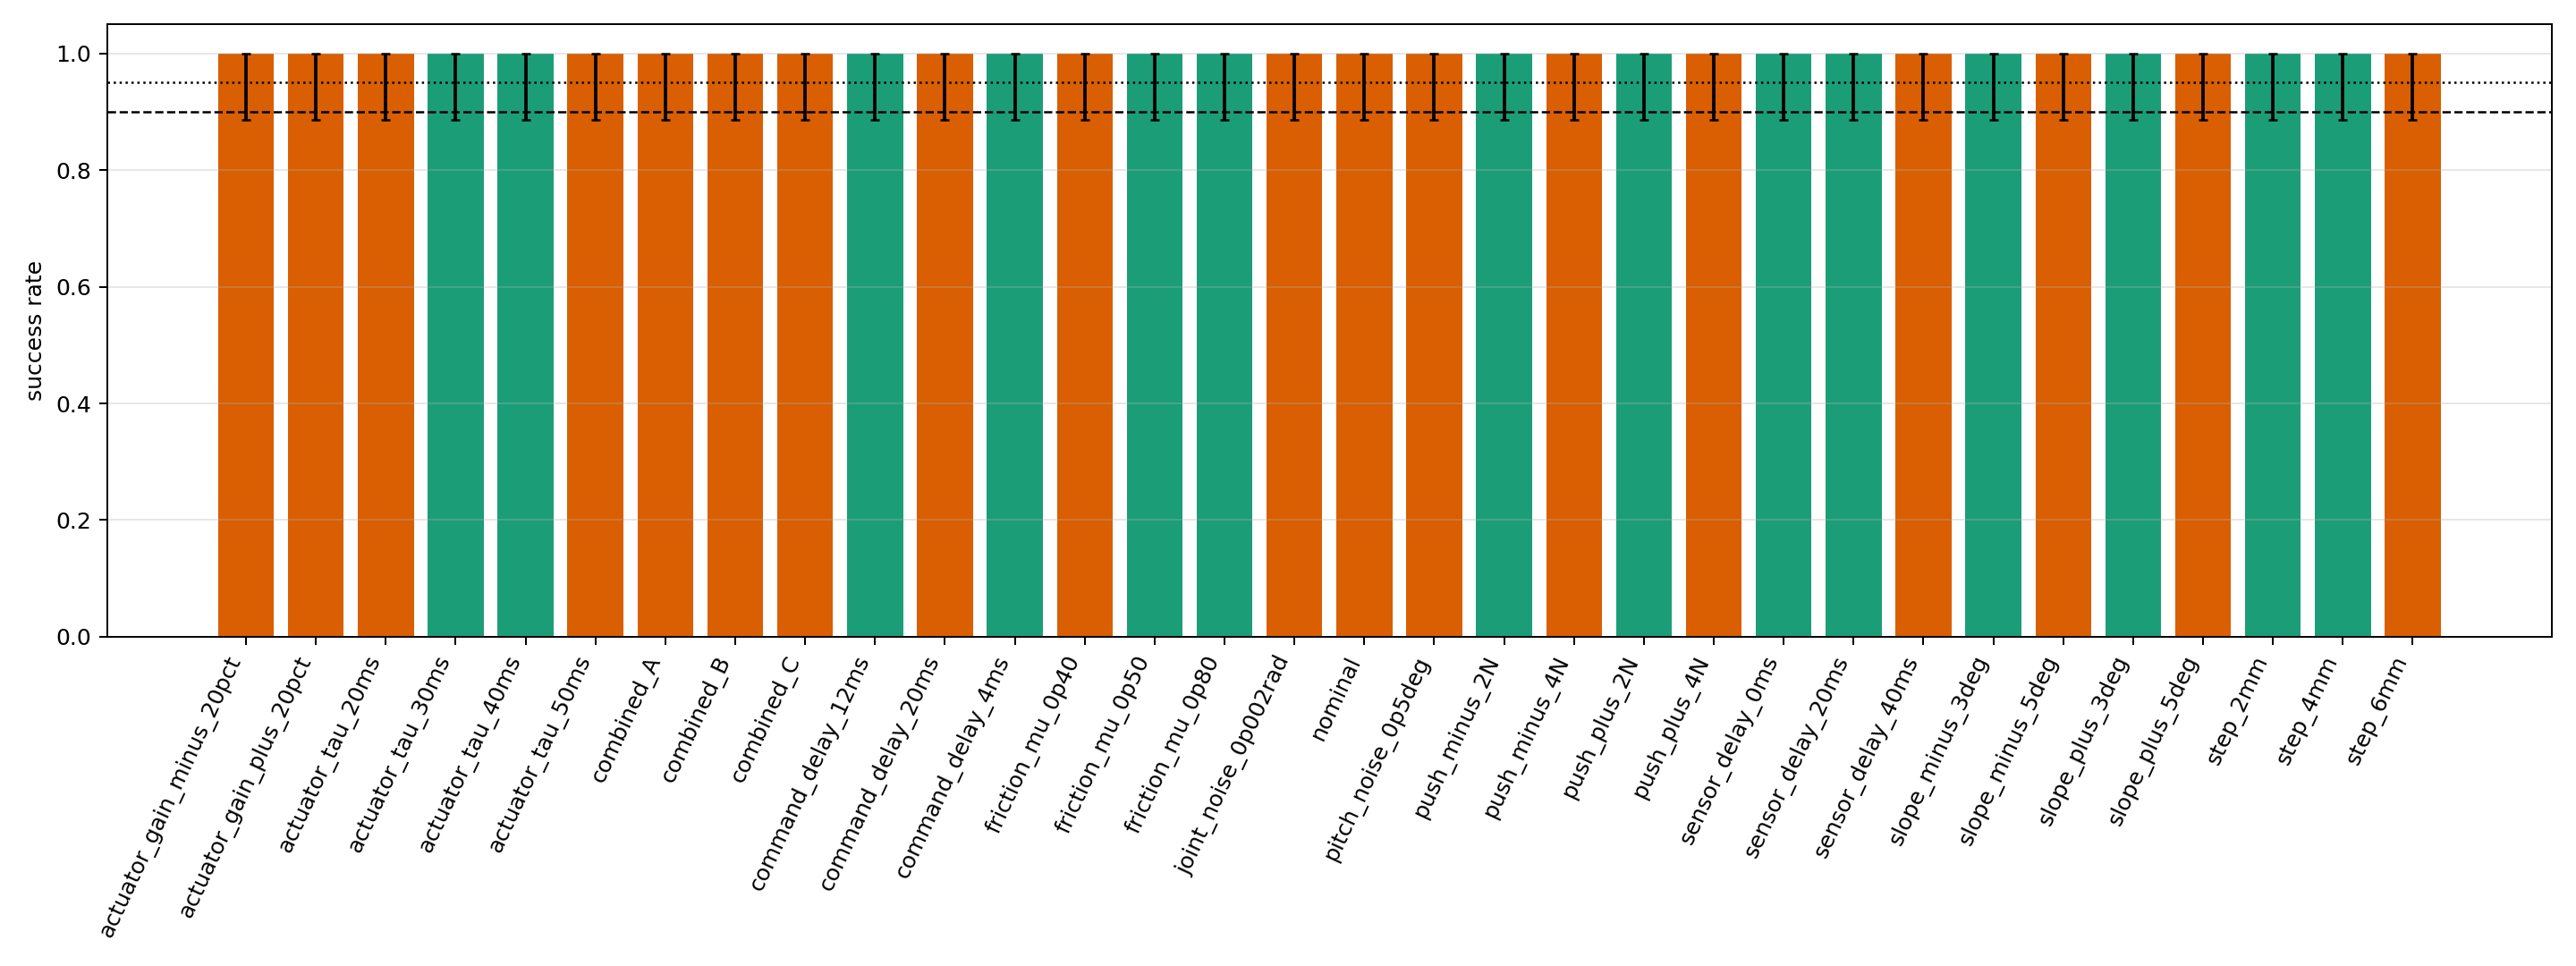
\includegraphics[width=0.92\linewidth]{fddp_multistep_robustness_matrix.png}%
}{\fbox{\parbox[c][4.0cm][c]{0.84\linewidth}{\centering 请将 \code{results/figures/fddp\_multistep\_robustness\_matrix.png} 上传到 Overleaf。}}}
\caption{Final 10-step FDDP/C2 robustness matrix。图用于快速看覆盖范围，正式结论仍以 YAML/CSV gate 为准。}
\end{figure}

\begin{warningbox}
允许的结论是：“在当前 planar model、position-actuator proxy、32 个预定义场景和 30 seeds 下，960/960 trials 通过。”不允许写成：“机器人在所有扰动下稳定”或“实机已经验证”。
\end{warningbox}

\section{E6 timing、safety 与 runtime-loadability}\label{sec:timing}

\subsection{Timing 到底测的是什么}

controller update rate 为 \SI{50}{Hz}，所以每次更新的 nominal deadline 是 \SI{20}{ms}。历史 E6 记录包含 4 个 conditions、每个 61 次 update，共 244 次；worst-condition p95 为 \SI{1.082}{ms}、observed maximum 为 \SI{1.508}{ms}，deadline misses 为 0。这说明当前 Python controller 在该机器和该短时 workload 下有明显计算余量，但样本太短，且不是 real-time operating system，因此不能称 hard real-time proof。

\begin{figure}[htbp]
\centering
\IfFileExists{e6_controller_timing_distribution.png}{%
 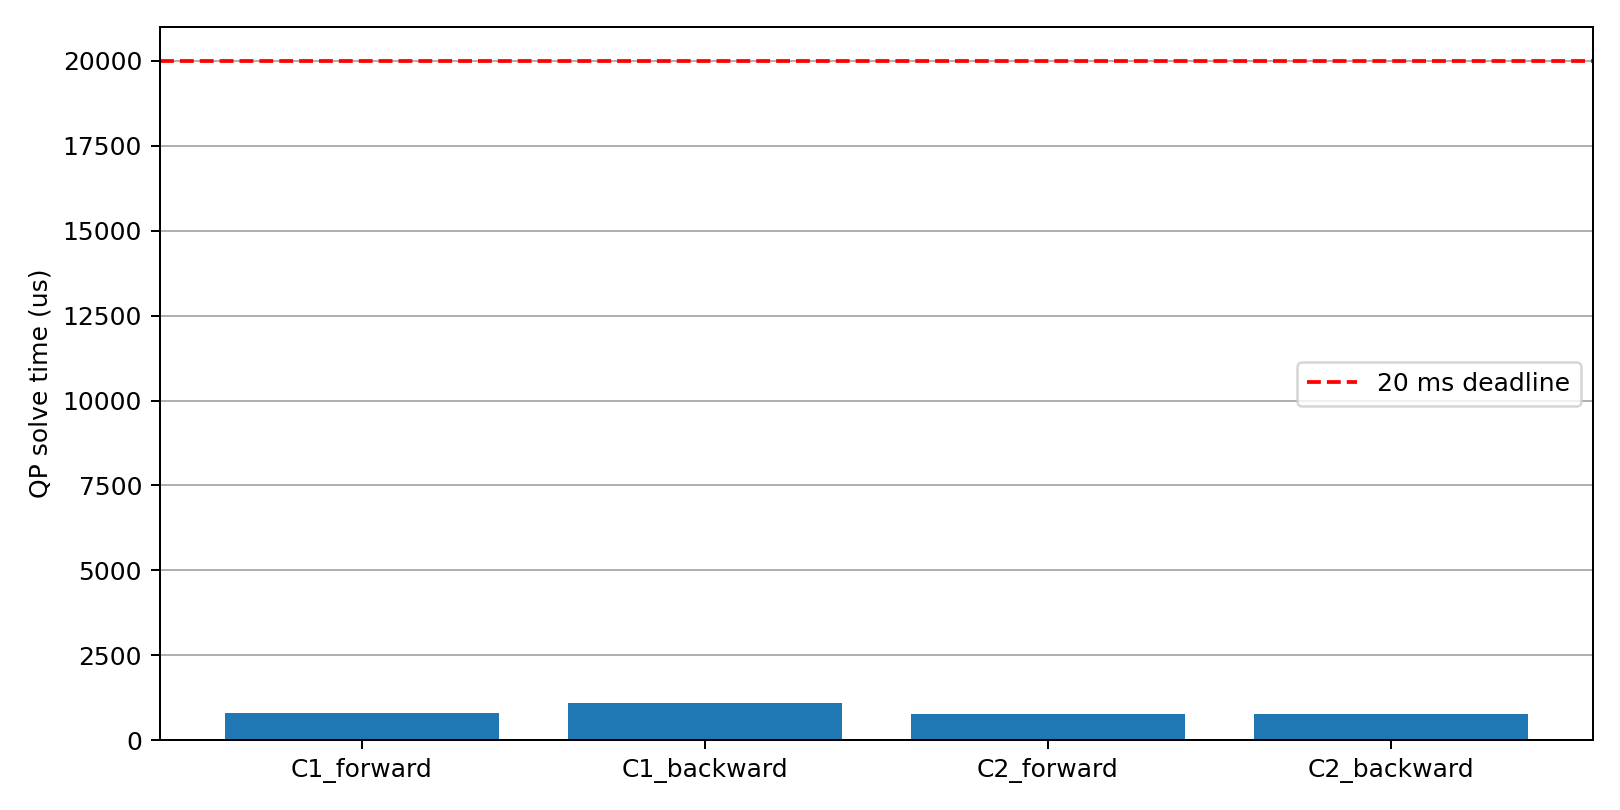
\includegraphics[width=0.84\linewidth]{e6_controller_timing_distribution.png}%
}{\fbox{\parbox[c][3.8cm][c]{0.78\linewidth}{\centering E6 timing distribution figure 未随本文件提供。}}}
\caption{历史 E6 controller execution-time distribution。它是 measured software timing，不是实时操作系统保证。}
\end{figure}

\subsection{为什么旧日志与新 safety evidence 看起来矛盾}

旧 E6 timing YAML 中 \code{fallback\_available=false}，这是当时 244-update benchmark 的历史状态，不能删改。随后项目增加了 runtime safety state machine，并通过 15 类 fault injection 验证了 \code{DEGRADED/FALLBACK/SAFE\_HOLD/FAILED} 路径。因此正确写法是：“旧 timing run 当时无 fallback；新 fault campaign 已验证 software fallback/state transitions。”两份证据时间和问题不同，并不矛盾。

\subsection{Runtime-loadability 与硬件的距离}

runtime-loadability 表示 nominal NPZ、controller parameters 和 command-generation code 能被 loader 正常加载，并能生成
\begin{equation}
 \bm q_{\rm cmd}=\bm q_{\rm ref}+\Delta\bm q
\end{equation}
形式的有限位置目标。它不表示已完成 ST3215 串口 round-trip、joint zero/direction calibration、电流/温度保护、通信 watchdog 实机联调，也不表示机器人已经站立或行走。

\begin{warningbox}
当前最准确的边界是：核心软件/仿真 acceptance chain 完成；15 类软件故障 containment 完成；历史短时 timing 有余量；100,000-update 长时 timing 和真实 hardware-in-the-loop 尚无正式证据。
\end{warningbox}

\section{从文件到结果的完整流程}\label{sec:pipeline}

\begin{enumerate}[label=\textbf{Step \arabic*:}]
 \item \textbf{Model preparation}：URDF 提供 Pinocchio/Crocoddyl dynamics；MJCF 提供 MuJoCo contact、actuator 与 sensor；consistency audit 维护映射 ledger。
 \item \textbf{Initial state}：构造 static double-support $\bm x_0=[\bm q_0,\bm v_0]$，检查 foot pose、CoM 与 joint limit。
 \item \textbf{FDDP problem}：按 DS/SS phase 建立 contact set、swing/support/CoM residual 和 regularisation。
 \item \textbf{Solve/continuation}：运行 backward/forward passes，记录 cost、stop、gap、regularisation、step length。
 \item \textbf{Gated export}：trajectory gates 通过才导出 nominal；multi-step 还要通过 normal force、friction 和 CoP gate。
 \item \textbf{C0 replay}：$q_{\mathrm{ref}}$ 经 position-command proxy 形成 baseline，并记录逐脚 natural-contact event。
 \item \textbf{FIR/AR identification}：用小 pulse 辨识 $\alpha\rightarrow$ pitch response，使用 holdout case 检查。
 \item \textbf{C1}：固定 reference clock，QP 每 \SI{20}{ms} 计算 $\alpha$，输出 $\bm q_{\mathrm{ref}}+\bm G\alpha$。
 \item \textbf{C2}：toe/heel observer 识别 event，更新 phase offset，再读取 retimed reference。
 \item \textbf{Batch/evidence}：固定 protocol、seed 和 gates，输出 CSV/YAML/PNG/GIF，并同时记录 failure。
 \item \textbf{Archive}：workspace 为 source of truth；验证后同步 D 盘、核对 SHA-256，再更新 Overleaf claim。
\end{enumerate}

\begin{table}[htbp]
\centering
\caption{主要目录与职责}
\begin{tabularx}{\linewidth}{@{}p{3.4cm}X@{}}
\toprule
目录 & 内容 \\
\midrule
\path{fddp/} & offline solver、contact schedule、trajectory gate 与 export \\
\path{simulation/} & MuJoCo position-command replay、natural-contact logging、animation \\
\path{mpc/} & FIR/AR identification、QP-MPC、C2 phase synchronisation、robustness scripts \\
\path{transfer/trajectories/} & 通过相应 export gate 的 nominal NPZ/YAML \\
\path{results/logs/} & machine-readable CSV/YAML 与 timing/event tables \\
\path{results/figures/} & plot 与 animation artifact \\
\path{tests/} & helper、loader、schedule、replay 与 regression tests \\
\path{docs/} & 实验记录、学习指南与 Overleaf 同步源 \\
\bottomrule
\end{tabularx}
\end{table}

最终 10-step disturbance scenario 的数据流是：FDDP nominal $\rightarrow$ MuJoCo actuator proxy $\rightarrow$ toe/heel 与 torso-pitch observation $\rightarrow$ C1 FIR-QP correction + C2 event-type local-leg retiming $\rightarrow$ reference-relative SafetyLimiter $\rightarrow$ $\bm q_{\mathrm{cmd}}$ $\rightarrow$ replay log。Task 6 已在同一协议中启用完整链；历史 CoM-shift、two-step 和 scripted experiments 仍应注明各自 branch，不能回填成 final integrated result。

\section{源 Word 文档 20 个问题逐题回答}\label{sec:questions}

本节保留问题原意并给出短答案。点击“详细解释”可返回前面的完整章节。原问题中的“13、15、16”引用了未保存在 Word 内的旧回答编号；本文按相邻问题语境分别映射为 parameter/gate rationale、validation rationale 和完整 pipeline，并明确这一解释。

\subsection{Q1：$n_q=13,n_v=12$ 是什么？}\label{q1}
Free-flyer configuration 是 3 translation + 4 quaternion，再加 6 joints，所以 $n_q=13$；velocity 是 6D base twist + 6 joint velocities，所以 $n_v=12$。\hyperref[sec:nqnv]{详细解释见第~\ref*{sec:nqnv}节}。

\subsection{Q2：MJCF 为什么使用 simplified planar base？}\label{q2}
因为研究对象只验证 sagittal $Y$--$Z$ motion 与 pitch $X$，planar root 移除 roll/yaw/lateral modes，降低 simulator 中与研究问题无关的自由度。但这也限制结论不能外推到 3D balance。\hyperref[sec:models]{见模型章节}。

\subsection{Q3：既然 MJCF 和 URDF 不完全一样，为什么引入 MJCF？}\label{q3}
URDF/Pinocchio 服务于 dynamics derivatives 与 FDDP；MJCF 原生支持 MuJoCo contact、actuator、sensor 和 replay。二者职责不同，必须 audit 而不是要求文本相同。\hyperref[sec:models]{见第~\ref*{sec:models}节}。

\subsection{Q4：为什么要 audit，怎样做？}\label{q4}
Audit 逐项核对 body mass/COM/inertia、joint axis/range/damping、geometry、collision、actuator 和 sensor，把差异分类。当前 154 ledger rows、0 unexpected mismatches，但 full equivalence 仍为 false。\hyperref[sec:models]{见第~\ref*{sec:models}节}。

\subsection{Q5：$q_{ref}$、$\Delta q$、$q_{cmd}$ 的单位是什么？}\label{q5}
三者均是 joint angle，单位 rad；$q_{cmd}=q_{ref}+\Delta q$。绘图可换成 degree，但计算和接口保持 rad。\hyperref[sec:signals]{见信号字典}。

\subsection{Q6：\code{dq\_ref} 可以详细解释吗？}\label{q6}
\code{dq\_ref} 是 nominal joint velocity，单位 rad/s；它不是 $\Delta q$。前者来自 FDDP state，后者来自 online MPC。\hyperref[sec:signals]{见信号字典}。

\subsection{Q7：为什么引入 6D contact，有依据吗？}\label{q7}
Rigid flat foot 需要固定 SE(3) placement，即 3 translation + 3 rotation。Crocoddyl multi-contact optimal control 和 humanoid locomotion 文献均使用这类 flat-foot contact abstraction\cite{mastalli2020crocoddyl,kuindersma2016optimization}。\hyperref[sec:contact]{见 contact 章节}。

\subsection{Q8：shooting 是什么，shooting gap 是什么？}\label{q8}
Shooting 把 trajectory 划成由 dynamics rollout 连接的 segments。Gap 是 stored next state 与 rollout next state 的 manifold difference；gap 0 表示 dynamics continuity，不代表所有 physical constraints 都通过。\hyperref[sec:node]{见 node 与 shooting 解释}。

\subsection{Q9：Node 是什么？左右单步现在成功了吗？怎样改进？}\label{q9}
Node 是一个 \SI{10}{\milli\second} dynamics/cost 单元。左右单步 physical gates 与 replay integrity 通过，但 first-order solver success 未通过；所以是“指定可行性通过、first-order convergence 未成功”。优先用 homotopy、scaling、better seed、derivative audit 和 boundary costs 改进。\hyperref[sec:node]{Node 解释}；\hyperref[sec:weights_results]{结果与改进}。

\subsection{Q10：当前 FDDP 是否完善？还能怎样优化？}\label{q10}
单步、两步、periodic cycle、10-step planning/contact、完整 natural-contact replay、integrated C1/C2-final、$\pm\SI{4}{N}$ 双方向 30-seed recovery、15 类 fault injection 和 960-trial robustness 已形成证据阶梯。尚缺的是 100,000-update 长时 timing、最终 fresh rerun/archive 和真实硬件 bench/standing/walking。\hyperref[sec:multistep]{见 multi-step 状态}。

\subsection{Q11：clearance 和 quintic progress 是什么，为什么用这个式子？}\label{q11}
Clearance 防止 swing foot 拖地；quintic $10r^3-15r^4+6r^5$ 让 position、velocity、acceleration 在两端连续且端点速度/加速度为 0。\hyperref[sec:quintic]{见第~\ref*{sec:quintic}节}。

\subsection{Q12：权重这样设置的表现如何，还能优化吗？}\label{q12}
当前权重使左右单步 physical gates 通过、两步达到 first-order convergence，更新后的 10-step contact gates 也通过；但单步 stop 仍约 $10^{-3}$。后续应继续做 residual normalisation、one-factor ablation、homotopy 与跨 phase robustness，而不是用一套权重宣称普适最优。\hyperref[sec:weights_results]{见权重与结果}。

\subsection{Q13：原回答“13”为什么这样设置，有什么参考依据？}\label{q13}
旧编号缺失，本文按上下文解释为 FDDP parameters/gates。依据不是某篇文献给出同一组数值，而是 DDP/FDDP weighted residual framework、SI scaling、physical safety threshold 与本项目 ablation/continuation evidence。任何数值都应写成 model-specific choice。\hyperref[sec:weights_results]{见第~\ref*{sec:weights_results}节}。

\subsection{Q14：原回答“15”为什么要做，结果如何？}\label{q14}
本文按上下文解释为 independent validation。原因是同一数据上 fit 和 test 会产生 optimistic conclusion；因此做 FIR holdout、C0/C1/phase-only/C2-final common-protocol comparison、contact gate、model audit、双方向 recovery、fault injection 和 960-trial matrix。旧的 C2 event skip、10-step smoke failure 与 scripted strong-push failure 均保留为 historical negative evidence；当前 final FDDP recovery 已达到 $\pm\SI{4}{N}$ 各 30/30，但仍只能在已定义的 simulation protocol 内表述。\hyperref[sec:balanced]{见 C1/holdout}，\hyperref[sec:evidence]{见 E1--E6}。

\subsection{Q15：原回答“16”的细流程图是什么？}\label{q15}
完整流程是 model/audit $\rightarrow x_0\rightarrow$ node/contact costs $\rightarrow$ FDDP solve $\rightarrow$ gated export $\rightarrow$ C0 replay $\rightarrow$ FIR identification $\rightarrow$ C1 $\rightarrow$ C2 $\rightarrow$ robustness/statistics/archive。\hyperref[sec:pipeline]{见完整流程}。

\subsection{Q16：C1 为什么用 fixed mapping？}\label{q16}
Fixed $G$ 把六关节 correction 压缩成一个经过 calibration 的协调 direction，使 FIR identification 与 online QP 维度足够小、timing 可控。代价是局部性，不能代表任意 contact mode 的全身最优 feedback。\hyperref[sec:mapping]{见 fixed mapping}。

\subsection{Q17：Balanced candidate 为什么这样选？}\label{q17}
Balanced 是历史 CoM-shift 的稳健基准；最终 10-step experiment 在相同模型和周期下复用 one-factor candidates，选择 \code{r\_low}，因为它使 C1 IAE 改善 10.79\% 并保持 peak/contact/height/correction gates。参数选择仍是 model-specific evidence，不是 global optimum。\hyperref[sec:balanced]{见 selection rationale}。

\subsection{Q18：holdout validation 是什么？}\label{q18}
留出未用于 identification 的 pulse/case 做 prediction test。当前 holdout 仍是局部、有限样本证据，支持 local generalisation，不支持广泛统计结论。\hyperref[sec:balanced]{见 C1 与 holdout 范围}。

\subsection{Q19：C2 怎样更新时间偏差？}\label{q19}
C2-final 对 left/right liftoff/touchdown 分别记忆 bounded predictive offset；fixed wall clock 继续服务 pitch baseline 和支撑腿，motion clock 只重定时下一 event 所属腿。这样 late liftoff 不会被准时 touchdown 抵消。\hyperref[sec:c2]{见公式与结果}。

\subsection{Q20：E1--E6 是什么？}\label{q20}
它们是从 FDDP convergence、C0、C1、FIR holdout、C2 mismatch 到 online timing/safety 的六组 evidence categories，不是六个算法。\hyperref[sec:evidence]{见证据矩阵}。

\section{怎样直接用于论文和 PPT}\label{sec:writing_ppt}

\subsection{论文建议结构}

论文叙事不要按脚本编号排列，而要按 research question 排列：
\begin{enumerate}
 \item \textbf{System and modelling}：解释 planar 6-DoF robot、URDF/Pinocchio/Crocoddyl 与 MJCF/MuJoCo 的消费者边界，以及 position-controlled servo interface。
 \item \textbf{Offline nominal generation}：说明 DS--SS contact schedule、periodic two-step、4/6/10-step continuation、planning/contact promotion gates。
 \item \textbf{Independent replay}：说明 actuator delay/lag/speed proxy、\SI{30}{ms} command advance、20-event matching 与 full replay acceptance。
 \item \textbf{Online controller}：先定义 C0/C1/phase-only/C2-final，再给出 FIR/AR/QP、reference-relative limiter 和 event-type local-leg synchronisation。
 \item \textbf{Results}：依次报告 planning/contact table、nominal replay figure、four-mode ablation table；把旧 smoke failure 和旧 global-phase failure 作为 design evolution，而不是当前结论。
 \item \textbf{Limitations}：明确 simulation-only、planar model、local FIR identification；说明 recovery/fault/statistical gates 已完成，而 100,000-update timing、最终归档和真实硬件仍未完成。
\end{enumerate}

论文中最安全的主结论句是：
\begin{quote}
The accepted ten-step FDDP nominal was replayed for \SI{10}{s} in MuJoCo through a position-actuator proxy, with 20/20 ordered contact events matched. Under the common disturbance protocol, C1 reduced pitch-error IAE by 10.79\% relative to C0, while C2-final reduced mean contact-timing error by 38.16\% relative to fixed-phase C1 without worsening peak pitch error.
\end{quote}
紧接着必须加一句：这些结果是 simulation evidence，不是 hardware walking evidence。

\subsection{论文图表最小集合}

\begin{table}[htbp]
\centering
\caption{建议进入论文正文的最小证据集合}
\begin{tabularx}{\linewidth}{@{}p{3.1cm}X X@{}}
\toprule
位置 & 图/表 & 回答的问题 \\
\midrule
Method & FDDP $\rightarrow$ replay $\rightarrow$ C0/C1/C2-final pipeline diagram & 每个模块负责什么，数据怎样流动 \\
Planning result & 10-step planning/contact gate table + contact-feasibility figure & nominal 是否数值/物理可接受 \\
Replay result & \code{fddp\_multistep\_nominal\_replay.png} & 独立 simulator 是否完整复现 nominal \\
Controller result & four-mode ablation table + \code{fddp\_multistep\_controller\_ablation.png} & C1/C2-final 是否分别带来预期改善 \\
Limitations & completed/pending table & 哪些 claim 已有证据，哪些不能写 \\
\bottomrule
\end{tabularx}
\end{table}

\subsection{组会或答辩 PPT 的 12 页主线}

\begin{enumerate}
 \item Title 与一句话目标：低成本 planar biped 的 offline nominal + online correction。
 \item Motivation：contact switching、model mismatch、servo delay 和 disturbance 为什么使 walking 困难。
 \item Robot/model boundary：6 joints、planar、position command、$\tau_{ref}$ analysis-only。
 \item Overall pipeline：FDDP $\rightarrow$ contact gate $\rightarrow$ MuJoCo $\rightarrow$ C0/C1/C2-final $\rightarrow$ runtime。
 \item FDDP formulation：只保留一张 cost/contact schedule 图和必要公式，不从长推导开始。
 \item 10-step planning/contact evidence：solver、clearance、CoM、friction、CoP。
 \item Full nominal replay：20/20 events、RMSE $1.124^\circ$、pitch $9.479^\circ$、height 97.9\%。
 \item Four controller modes：用 2$\times$2 table 区分 correction 和 phase synchronisation。
 \item Engineering findings：30 ms advance、reference-relative limiter、20 ms FIR alignment、event-type local-leg retiming。
 \item Ablation result：C1 IAE $-10.79\%$；C2 timing error $-38.16\%$；五项 checks passed。
 \item Software evidence：展示 $\pm\SI{4}{N}$ 各 30/30、15 类 fault、32 场景与 960/960，并列出 machine-readable YAML/CSV。
 \item Honest conclusion：当前定义的核心软件/仿真验收链完成；100,000-update timing、最终归档和真实硬件仍是边界。
\end{enumerate}

\section{已完成、仍缺什么与“是否只剩硬件”}\label{sec:gaps}

\begin{table}[htbp]
\centering
\caption{截至 2026 年 7 月 19 日的项目状态}
\begin{tabularx}{\linewidth}{@{}p{3.7cm}p{1.7cm}X@{}}
\toprule
工作包 & 状态 & 当前证据或剩余边界 \\
\midrule
10-step planning/contact & \pass & promoted reference；solver、trajectory 与 planar contact gates passed \\
Full 10-step MuJoCo replay & \pass & \SI{10}{s}、20/20 ordered events、integrity true \\
C0/C1/phase-only/C2-final & \pass & five acceptance checks passed；C1 IAE $-10.79\%$，C2 timing error $-38.16\%$ \\
$\pm\SI{4}{N}$ recovery & \pass & selected \code{fir\_fast}；forward 30/30、backward 30/30 \\
Runtime safety/fault injection & \pass & 15 类 fault accepted；commands finite、within limits、rate-bounded \\
FDDP-gait robustness statistics & \pass & 32 scenarios、30 seeds、960/960，aggregate gate passed \\
Long-duration timing & \partialstatus & 历史 244 updates 无 miss；100,000-update formal benchmark 尚无证据 \\
Reproducibility/archive & \partialstatus & machine-readable artifacts 已有；最终 fresh rerun、hash/Overleaf bundle 可继续整理 \\
Real hardware & \pending & 串口、舵机标定、保护架静态测试、HIL、站立和行走尚未完成 \\
\bottomrule
\end{tabularx}
\end{table}

\begin{evidencebox}
如果“软件和仿真完成”的定义是当前项目已经明确写下的 core acceptance gates，那么答案是\textbf{是：核心链条已完成，下一大阶段是硬件}。如果按可交付工程系统的最高标准，还应在上硬件前补做 100,000-update timing、fresh clean-environment rerun 与最终 hash/archive。这些是 assurance 与交付收尾，不是新的核心 walking algorithm。
\end{evidencebox}

\subsection{上硬件前的建议顺序}

\begin{enumerate}
 \item \textbf{长时软件检查：}运行 100,000 updates，记录 p99、maximum、deadline miss、memory growth 和 fallback transitions。
 \item \textbf{可复现归档：}从干净环境执行 planning $\rightarrow$ replay $\rightarrow$ controller $\rightarrow$ recovery/fault/robustness，固定 interpreter、seed、config 与 SHA-256。
 \item \textbf{无负载 bench：}逐个舵机确认 ID、方向、零位、角度/速度限制、掉线行为和 emergency stop。
 \item \textbf{保护架静态测试：}先双脚支撑的小幅 $q_{\rm cmd}$，再验证传感器、串口延迟、watchdog 和 safe hold。
 \item \textbf{hardware-in-the-loop：}保持机器人受支撑，播放低速 nominal 并比较真实 joint/pitch/contact 与 MuJoCo。
 \item \textbf{逐步行走：}从单步、两步到十步，每一级重新定义 hardware gate；不能直接把 simulation threshold 原样当作硬件安全阈值。
\end{enumerate}

\begin{warningbox}
真实硬件阶段最危险的假设是“position command 有限，所以实机安全”。实际舵机方向反了、零位偏了、电源压降或串口丢包，都可能让有限角度命令变成危险动作；因此 bench 和保护架测试必须在自由行走之前。
\end{warningbox}

\section{零基础术语表}\label{sec:glossary}

\begin{longtable}{@{}p{0.25\linewidth}p{0.63\linewidth}@{}}
\toprule
术语 & 在本项目中的通俗解释 \\
\midrule
\endhead
Biped & 双足机器人；本项目只研究前后方向的 planar motion。\\
DoF & Degree of Freedom，自由度；这里有六个可驱动腿部关节。\\
Sagittal plane & 矢状面，即从侧面看的前后--上下平面。\\
Configuration $\bm q$ & 描述机器人“现在摆成什么姿势”的位置变量。\\
Velocity $\bm v$ & 描述姿势变化有多快。\\
State $\bm x$ & 通常把 $\bm q$ 与 $\bm v$ 合在一起。\\
Control $\bm u$ & 优化器选择的输入；FDDP 中近似为力矩，硬件接口中不是直接发送它。\\
Nominal trajectory & 在没有额外扰动时希望机器人遵循的参考动作。\\
Reference $\bm q_{\rm ref}$ & nominal 中的关节角度序列。\\
Correction $\Delta\bm q$ & 在线控制器为了纠偏加上的小角度。\\
Command $\bm q_{\rm cmd}$ & 真正送往位置执行路径的目标角度，等于 reference 加 correction。\\
URDF & 供 Pinocchio/Crocoddyl 使用的机器人结构与惯量描述。\\
MJCF & 供 MuJoCo 使用的模型，能直接描述接触、传感器和执行器。\\
Pinocchio & 快速计算运动学、刚体动力学和导数的库。\\
Crocoddyl & 构造并求解多接触最优控制问题的库。\\
MuJoCo & 做带接触 forward simulation 的独立物理引擎。\\
Forward dynamics & 已知状态和输入，向前计算下一时刻状态。\\
Optimal control & 在动力学约束下寻找使总代价最小的一串状态和输入。\\
DDP & Differential Dynamic Programming，用局部二次近似迭代改进整条轨迹。\\
FDDP & Feasibility-driven DDP，允许中间 trajectory 暂时不连续，并同时推进可行性与代价。\\
Shooting node & 轨迹上的一个离散时间单元。\\
Shooting gap & 相邻 node 储存状态与 dynamics rollout 状态之间的差。\\
Residual & “当前量与目标量差多少”，例如脚位置误差或躯干角误差。\\
Cost weight & 决定某类 residual 在优化中有多重要的系数。\\
Contact schedule & 哪只脚在什么时间支撑、抬起和落地的计划。\\
DS/SS & Double Support/Single Support，双脚支撑/单脚支撑。\\
6D contact & 约束平脚的三维位置和三维方向。\\
CoM & Centre of Mass，质心；其位置影响是否能保持支撑。\\
CoP & Centre of Pressure，压力中心；应留在支撑区域内。\\
Friction utilisation & 已使用摩擦相对于摩擦极限的比例。\\
Replay & 把 reference 交给独立仿真器重新执行，而不是再次求解。\\
C0 & 不加在线 correction 的基线。\\
FIR & Finite Impulse Response，用有限个过去输入预测当前/未来响应。\\
AR & Auto-Regressive，用过去输出预测系统自然变化。\\
MPC & Model Predictive Control，反复预测未来、优化一段输入但只执行第一步。\\
QP & Quadratic Program，二次目标加线性/box constraints 的优化问题。\\
Receding horizon & 每个控制周期向前移动预测窗口并重新求解。\\
IAE & Integral Absolute Error，绝对误差随时间的积分；越小通常表示累计偏差越小。\\
Peak error & 整段试验中最大的绝对误差。\\
Settling time & 误差进入并保持在允许带内所需时间。\\
Phase & 当前 reference 播放到步态周期的哪个位置。\\
Contact synchronisation & 用真实 liftoff/touchdown 修正 reference phase。\\
Debounce & 接触信号需持续一小段时间才认定状态改变，避免抖动。\\
Limiter & 限制命令幅值与变化速度，防止不合理跳变。\\
Fallback & 在线优化不可用时退回更简单、可预测的 C0 path。\\
Fault injection & 人为制造坏测量、坏事件或坏文件，检查程序怎样响应。\\
Scenario & 一组固定测试条件，例如摩擦、坡度或 push。\\
Seed & 可复现随机扰动的编号。\\
Acceptance gate & 试验前定义的通过条件，避免看完结果再改标准。\\
Ablation & 每次只增加或去掉一个模块，判断改善来自哪里。\\
Holdout & 不参与辨识/调参的数据，用于独立检查。\\
Wilson interval & 二项成功率的置信区间，小样本时比只报百分比更诚实。\\
Runtime-loadability & 文件和参数能被执行程序加载并生成命令；不等于实机走路。\\
Hard real-time & 每次计算都必须在 deadline 前结束的系统保证；当前尚未证明。\\
\bottomrule
\end{longtable}

\section{代码与证据文件索引}\label{sec:file_index}

\begin{longtable}{@{}p{0.36\linewidth}p{0.52\linewidth}@{}}
\toprule
路径 & 用途 \\
\midrule
\endhead
\path{fddp/04a_solve_fddp_single_step_left_swing.py} & 左脚单步 schedule、cost、gates 与 export。\\
\path{fddp/04c_solve_fddp_two_step_alternating.py} & 两步交替 FDDP。\\
\path{fddp/05a_solve_fddp_periodic_cycle.py} & periodic cycle 与 boundary homotopy。\\
\path{fddp/05b_solve_fddp_multistep_continuation.py} & 4/6/10-step planning continuation。\\
\path{fddp/05c_report_fddp_multistep_contact_feasibility.py} & force/friction/CoP/slip report 与 final promotion gate。\\
\path{simulation/03p_replay_fddp_single_step_mujoco.py} & 单步 position-command replay。\\
\path{simulation/03r_replay_fddp_two_step_alternating_mujoco.py} & 两步 replay。\\
\path{simulation/03u_replay_fddp_multistep_mujoco.py} & Final 10-step full replay、event matching 与 unchanged acceptance gates。\\
\path{mpc/multistep_controller.py} & C0/C1/phase-only/C2-final 共用 position-command interface。\\
\path{mpc/18_validate_fddp_multistep_c2_final.py} & Four-mode common-protocol ablation 与 final acceptance。\\
\path{mpc/19_identify_fddp_multistep_fir.py} & 薄适配器：复用 mpc/16 辨识实现并对齐 10-step/20 ms。\\
\path{mpc/19_tune_fddp_multistep_push_recovery.py} & 复用 final pipeline 做 $\pm\SI{4}{N}$、30-seed recovery selection。\\
\path{mpc/20_run_multistep_fault_injection.py} & 15 类 runtime/startup fault 与安全状态验证。\\
\path{mpc/21_run_fddp_multistep_robustness_matrix.py} & 32 场景、960-trial final robustness matrix。\\
\path{mpc/07_run_reference_aligned_fir_qp_mpc_sweep.py} & C1 mapping、FIR-QP 与 common candidate sweep。\\
\path{mpc/08_run_contact_phase_synchronised_fir_qp_mpc.py} & C2 observer 与 bounded phase update。\\
\path{mpc/14_validate_fddp_two_step_natural_contact_c2.py} & Two-step natural-contact C2。\\
\path{mpc/17_run_fddp_two_step_c1_parameter_ablation.py} & Balanced 周围 one-factor ablation。\\
\path{results/logs/fddp_multistep_nominal_replay.yaml} & Full replay metrics、20-event integrity 与 command-advance provenance。\\
\path{results/logs/fddp_multistep_controller_ablation.yaml} & Final four-mode metrics、thresholds、five checks 与 integrity。\\
\path{results/logs/fddp_multistep_recovery_selection.yaml} & recovery candidate、$\pm4$ N 各 30/30 与 bounded-footstep claim boundary。\\
\path{results/logs/fddp_multistep_fault_injection.yaml} & 15 类 fault、state transition 与 command safety checks。\\
\path{results/logs/fddp_multistep_robustness_summary.yaml} & 32 场景、960/960 与 aggregate acceptance。\\
\path{tests/test_fddp_multistep_*.py} & Planning/replay/controller/identification regression contracts。\\
\path{model/02_audit_urdf_mjcf_consistency.py} & 154-row consistency ledger。\\
\path{results/logs/*.yaml,*.csv} & Machine-readable metrics 与 diagnostics。\\
\path{docs/2026-07-13/14_*.md} & Commands、thresholds、results、failures 与 claim boundary。\\
\bottomrule
\end{longtable}

\section{组会与答辩：一页、三分钟和十分钟怎样讲}\label{sec:oral}

\subsection{一页/一分钟版本}

\begin{quote}
本项目为 6-DoF、position-controlled planar biped 建立了“offline FDDP nominal planning + MuJoCo independent replay + online FIR-QP-MPC pitch correction + contact-phase synchronisation”的控制链。Final 10-step nominal 在 \SI{10}{s} replay 中匹配 20/20 contact events；C1 相对 C0 将 pitch IAE 降低 10.79\%，C2-final 相对 fixed-phase C1 将 contact-timing error 降低 38.16\%。随后 $\pm\SI{4}{N}$ 双方向 recovery 均为 30/30，15 类 fault injection 通过，32 场景共 960/960 trials 通过。结论限定为 planar position-command simulation；长时 timing 与真实硬件尚未验证。
\end{quote}

这页配四张证据即可：overall pipeline、10-step replay、four-mode ablation、robustness matrix。数字旁边标出 YAML 文件名，避免只给漂亮曲线。

\subsection{三分钟版本}

\begin{enumerate}
 \item \textbf{问题（30 秒）：}低成本位置舵机双足机器人既有接触切换，又有模型/延迟误差；单纯播放轨迹很难抵抗 pitch 与 contact timing mismatch。
 \item \textbf{方法（60 秒）：}FDDP 离线负责 nominal；MuJoCo 独立重放；C0 是基线；C1 用 pulse 辨识 FIR，再由小 QP 求 $\alpha$ 并形成 $\Delta q=G\alpha$；C2 用 toe/heel event 对下一局部腿的 reference 重新计时。
 \item \textbf{结果（60 秒）：}讲 20/20 events、IAE $-10.79\%$、timing error $-38.16\%$、$\pm4$ N 各 30/30、15 faults 和 960/960。
 \item \textbf{边界（30 秒）：}planar、simulation-only、position actuator proxy；100,000-update timing 和硬件 bench/standing/walking 尚未完成。
\end{enumerate}

\subsection{十分钟版本}

建议按“问题 $\rightarrow$ 为什么分层 $\rightarrow$ 每层证据 $\rightarrow$ 边界”讲，而不是按文件名讲：

\begin{enumerate}
 \item Robot 和 position-servo boundary；
 \item 为什么需要 URDF 与 MJCF 两套模型；
 \item 一般 FDDP 流程与本项目 contact-aware、gated continuation 流程；
 \item 单步、两步、periodic、十步的证据阶梯；
 \item 为什么 MuJoCo replay 是独立验证；
 \item C0、C1、C2 的 ablation 逻辑；
 \item FIR、AR、QP 的直觉和 $q_{\rm cmd}=q_{\rm ref}+G\alpha$；
 \item contact event synchronisation 为什么只重定时局部腿；
 \item recovery、fault injection 和 960-trial matrix；
 \item 当前能说什么、不能说什么、硬件阶段怎样推进。
\end{enumerate}

\subsection{导师最可能追问的九个问题}

\begin{enumerate}
 \item \textbf{为什么不用 FDDP 直接在线算？} 当前目标是低成本位置接口和 \SI{50}{Hz} 小型 online correction；完整 nonlinear solve 更重，且硬件不直接接收 torque。
 \item \textbf{为什么 C1 只有一个 $\alpha$？} 用 fixed $G$ 保持辨识和 QP 小而可解释；代价是局部性，已作为限制说明。
 \item \textbf{为什么需要 C2？} C1 修 pitch amplitude，不会自动修正 liftoff/touchdown 时间；两者处理不同误差。
 \item \textbf{MuJoCo 与规划模型不同是不是缺点？} 正是为了暴露 model mismatch；一致性 audit 负责区分预期差异和错误。
 \item \textbf{960/960 是否太完美？} 它只表示预定义 deterministic/stochastic proxy gates 全过；仍报告场景范围、seed 和 soft-contact penetration，不外推到硬件。
 \item \textbf{台阶是否真的碰到了？} 障碍几何已改为 toe 前方 \SI{5}{mm}，90/90 step trials 检测到接触。
 \item \textbf{强推失败历史去哪了？} 保留为 scripted-gait negative evidence；final FDDP pipeline retune 后 $\pm4$ N 各 30/30。
 \item \textbf{能否说软件全部完成？} 可说 core software/simulation acceptance chain 完成；long-duration timing、fresh archive 和 hardware integration 未完成。
 \item \textbf{你的核心贡献是什么？} 不是发明全新 FDDP，而是把 contact-aware planning、position-command replay、轻量 pitch MPC、event retiming 与可复核 acceptance evidence 集成为一条适合低成本 planar biped 的流程。
\end{enumerate}

\section{结语：最安全的总述}

本项目已经从模型一致性、离线 FDDP nominal、完整 MuJoCo position-command replay，推进到 C0/C1/C2-final、双方向强推恢复、软件故障 containment 与 960-trial statistical robustness。最重要的思路不是堆叠算法名字，而是让每一层只回答一个问题，并用下一层独立证据检查上一层的假设。当前可以说“定义范围内的核心软件与仿真链完成”；不能说“已证明三维稳定”“hard real-time 已证明”或“真实硬件已经自主行走”。

\begin{thebibliography}{9}

\bibitem{jacobson1970differential}
David H. Jacobson and David Q. Mayne.
\newblock \emph{Differential Dynamic Programming}.
\newblock Elsevier, 1970.

\bibitem{mayne2000constrained}
David Q. Mayne, James B. Rawlings, Christopher V. Rao, and Pierre O. M. Scokaert.
\newblock Constrained Model Predictive Control: Stability and Optimality.
\newblock \emph{Automatica}, 36(6):789--814, 2000.

\bibitem{todorov2012mujoco}
Emanuel Todorov, Tom Erez, and Yuval Tassa.
\newblock MuJoCo: A Physics Engine for Model-Based Control.
\newblock In \emph{IEEE/RSJ IROS}, pages 5026--5033, 2012.

\bibitem{carpentier2019pinocchio}
Justin Carpentier, Florian Valenza, Nicolas Mansard, et al.
\newblock The Pinocchio C++ Library: A Fast and Flexible Implementation of Rigid Body Dynamics Algorithms and Their Analytical Derivatives.
\newblock In \emph{IEEE/SICE SII}, pages 614--619, 2019.

\bibitem{mastalli2020crocoddyl}
Carlos Mastalli, Rohan Budhiraja, Wolfgang Merkt, et al.
\newblock Crocoddyl: An Efficient and Versatile Framework for Multi-Contact Optimal Control.
\newblock In \emph{IEEE ICRA}, pages 2536--2542, 2020.

\bibitem{kuindersma2016optimization}
Scott Kuindersma, Robin Deits, Maurice Fallon, et al.
\newblock Optimization-Based Locomotion Planning, Estimation, and Control Design for the Atlas Humanoid Robot.
\newblock \emph{Autonomous Robots}, 40(3):429--455, 2016.

\bibitem{tassa2014control}
Yuval Tassa, Tom Erez, and Emanuel Todorov.
\newblock Control-Limited Differential Dynamic Programming.
\newblock In \emph{IEEE ICRA}, pages 1168--1175, 2014.

\end{thebibliography}

\end{document}
